\section{Effektivitet af cuts}
\begin{frame}{Effekten af cuts}
	Hvordan ser usorteret data ud?\\
	\begin{figure}
		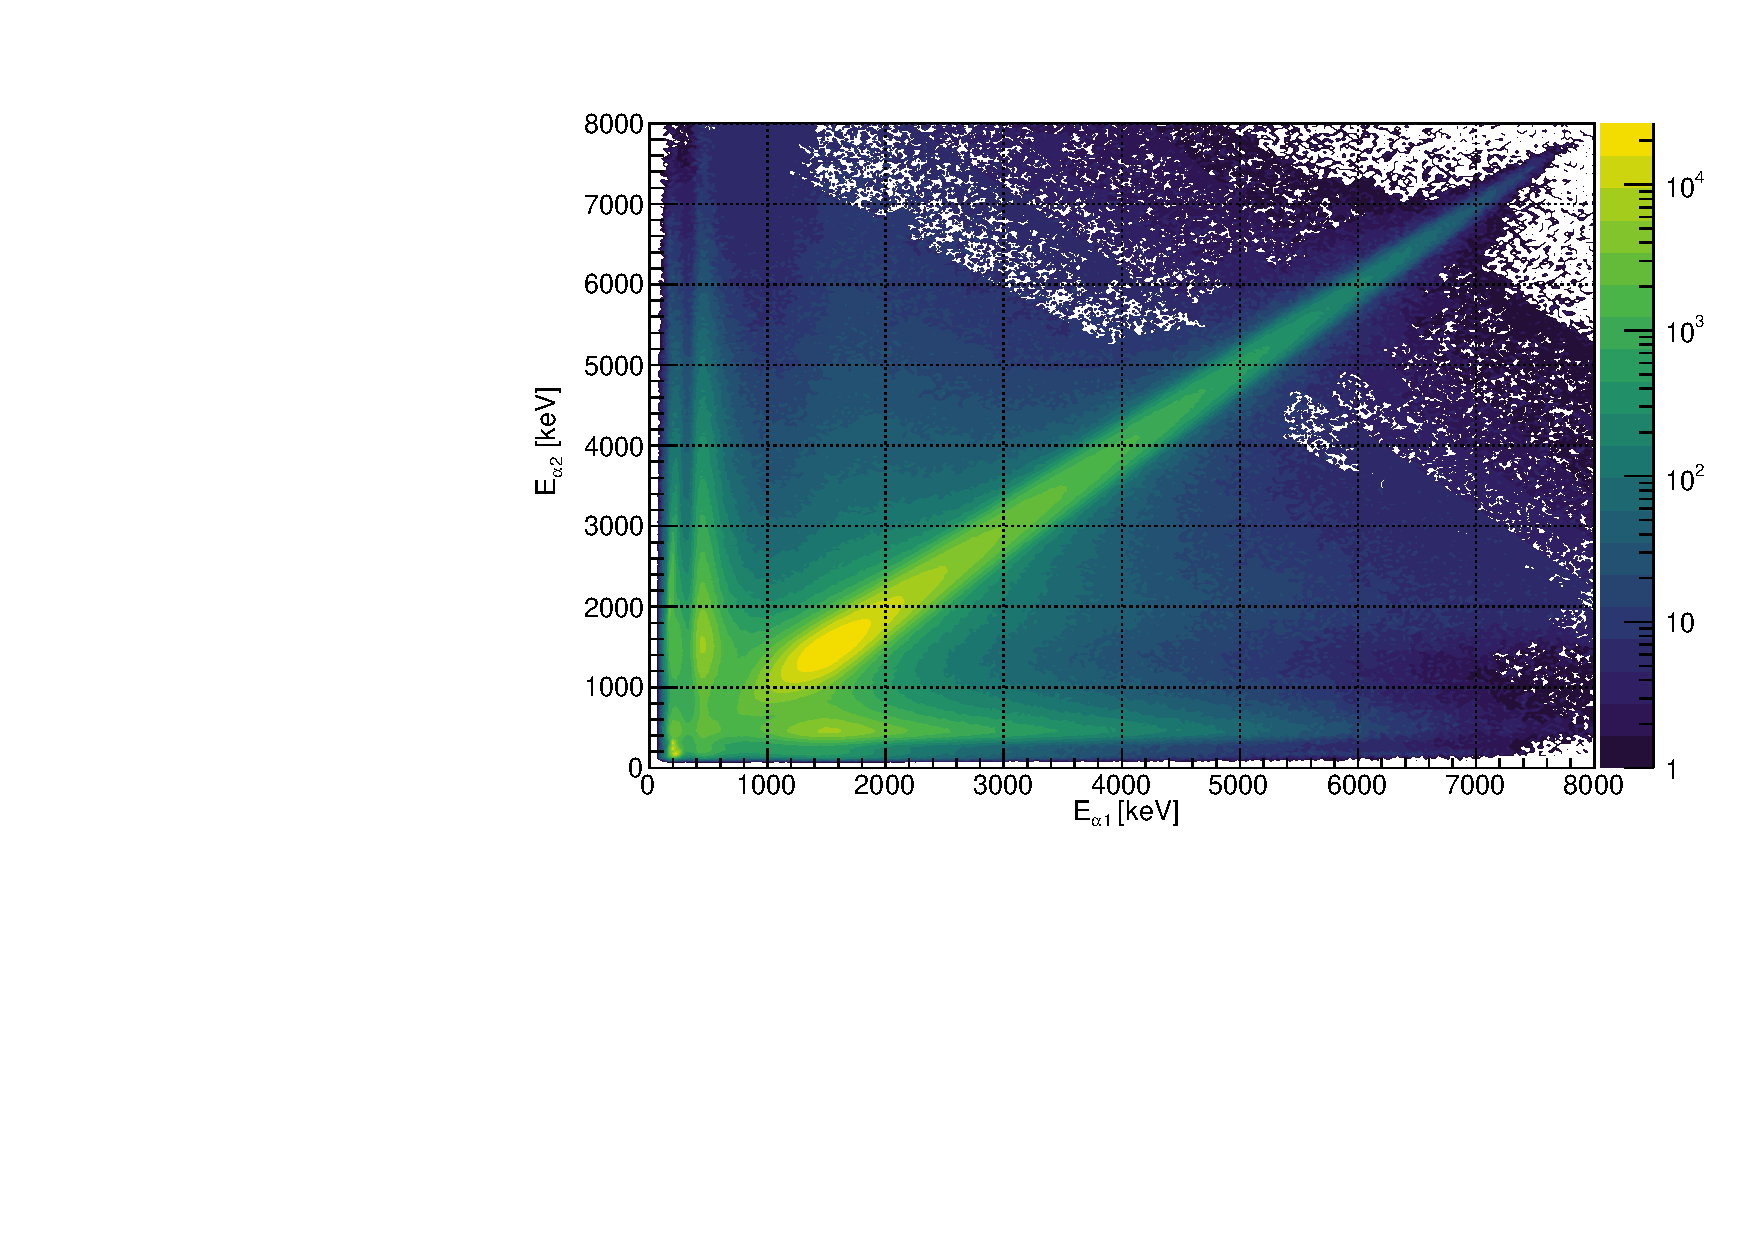
\includegraphics[width=0.7\columnwidth]{../figures/EENoCuts.pdf}
	\end{figure}
\end{frame}

\begin{frame}{Effekten af vinkel cut}
	Indbyrdes vinkel på maksimalt $161\degree$\\
	\begin{figure}
		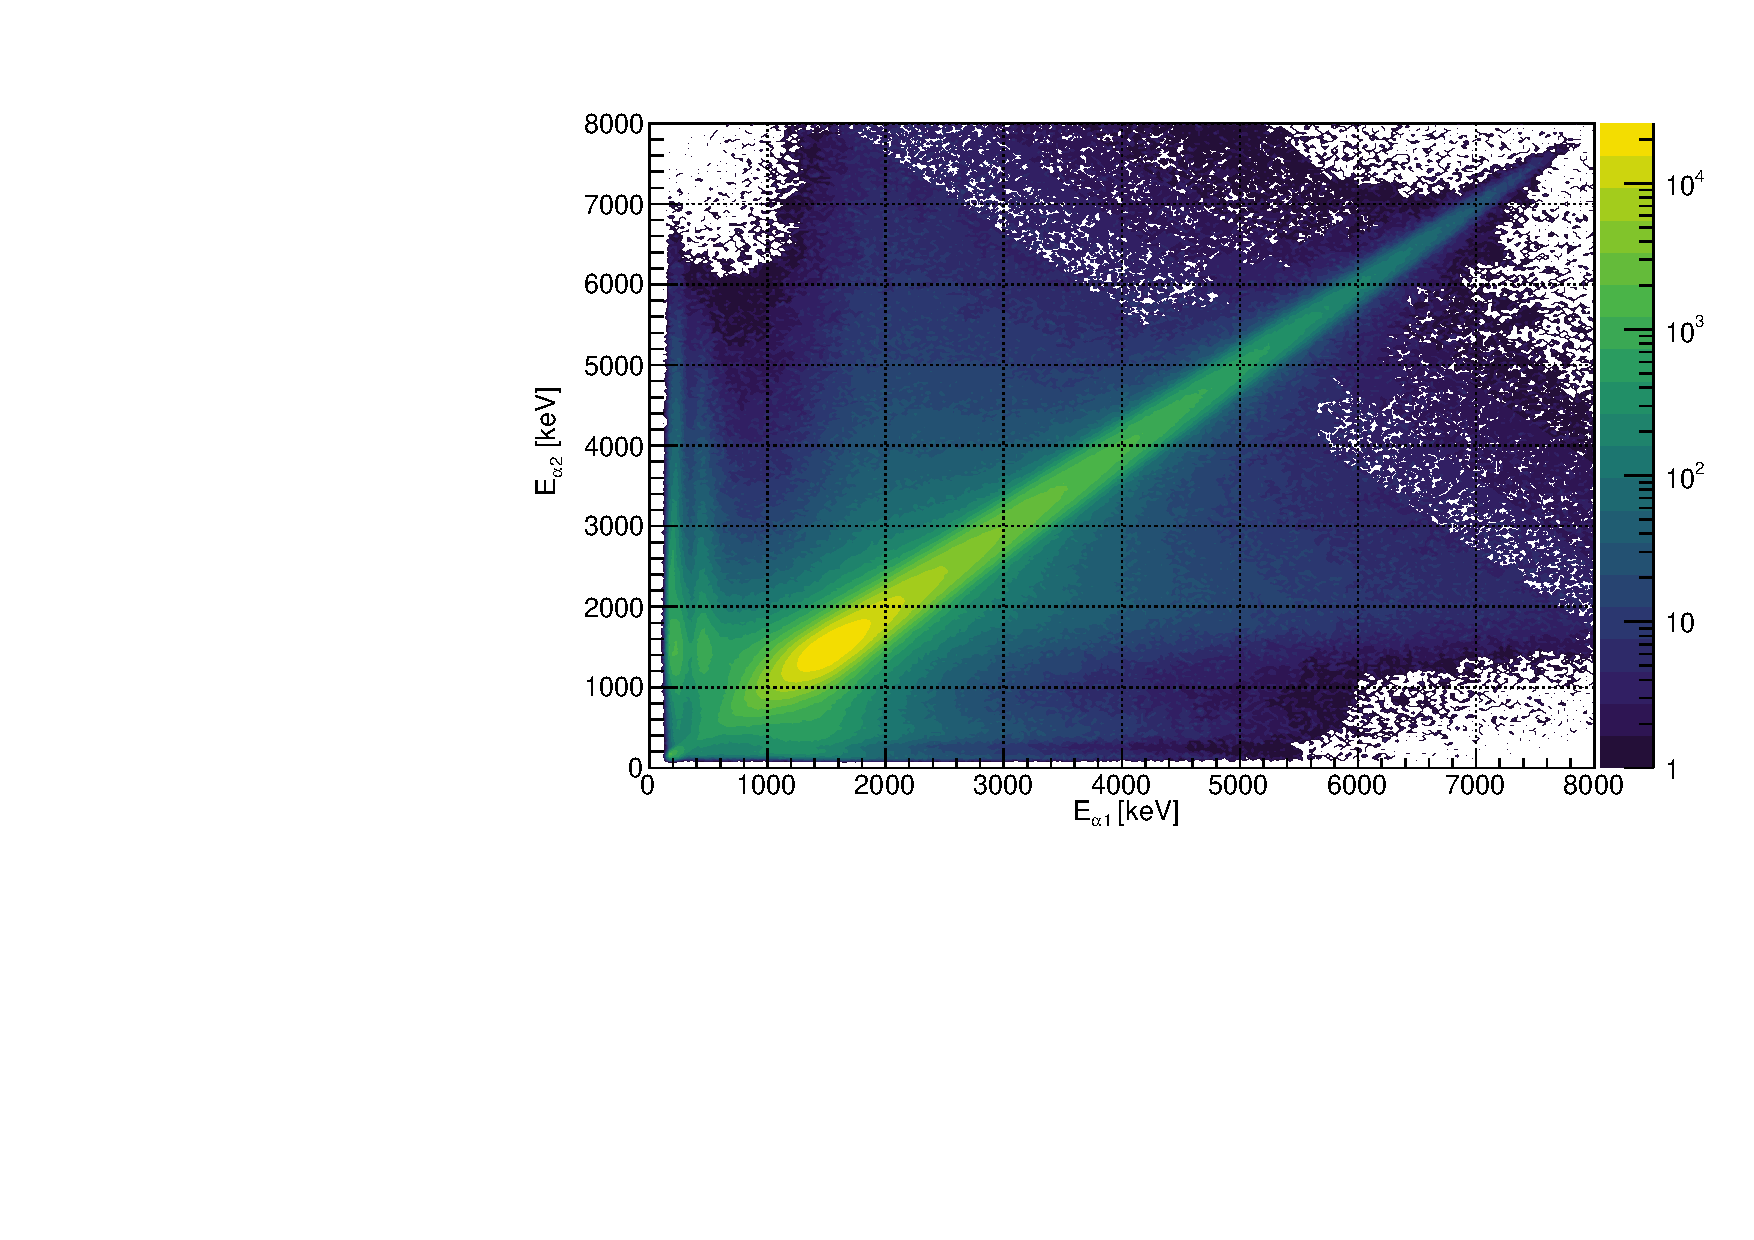
\includegraphics[width=0.7\columnwidth]{../figures/EEAngleCut.pdf}
	\end{figure}
\end{frame}

\begin{frame}{Effekten af impuls cut}
	Total impuls på maksimalt \SI{40}{MeV/c}
	\begin{figure}
		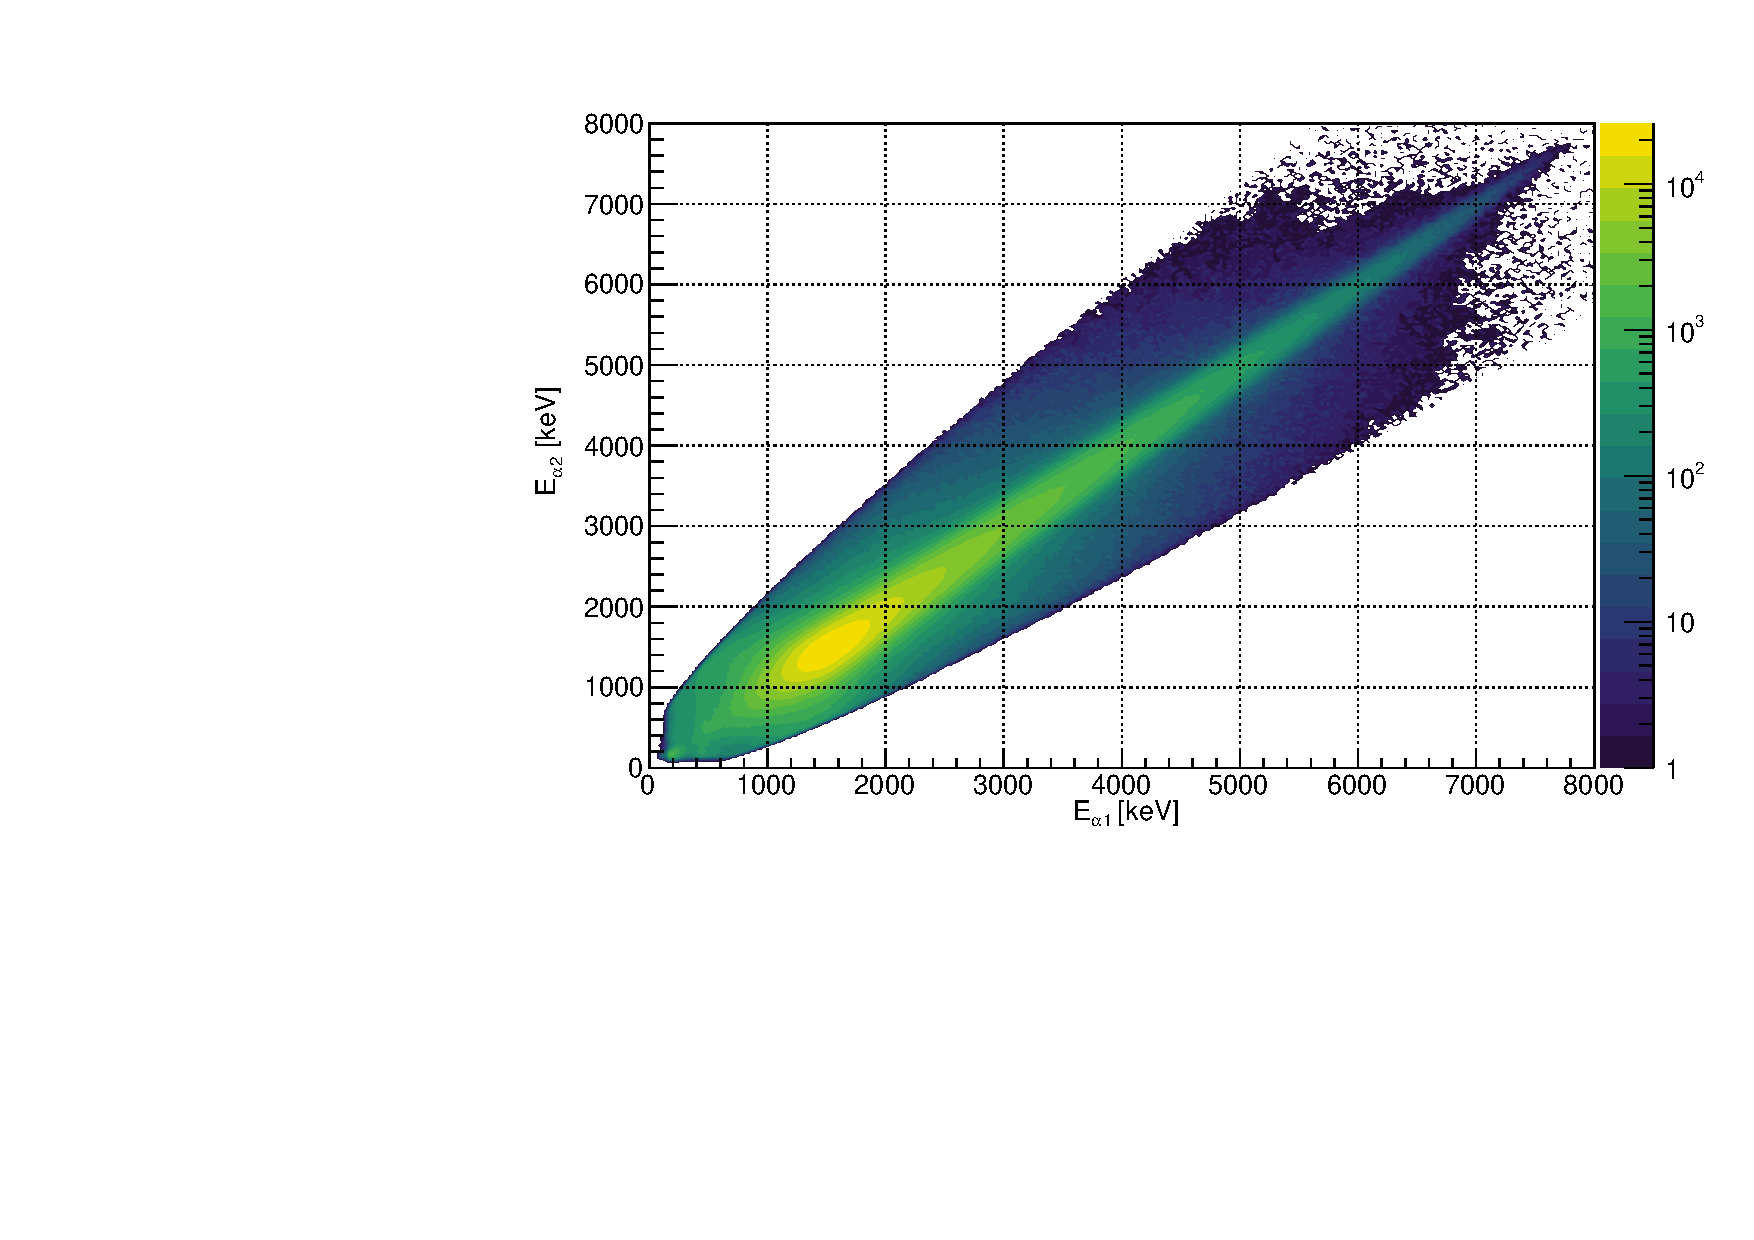
\includegraphics[width=.7\columnwidth]{../figures/EEMomentumCut.pdf}
	\end{figure}
\end{frame}

\begin{frame}{Effekten af \be-multiplicitet cut}
	Minimum 1 \be-partikel i et event
	\begin{figure}
		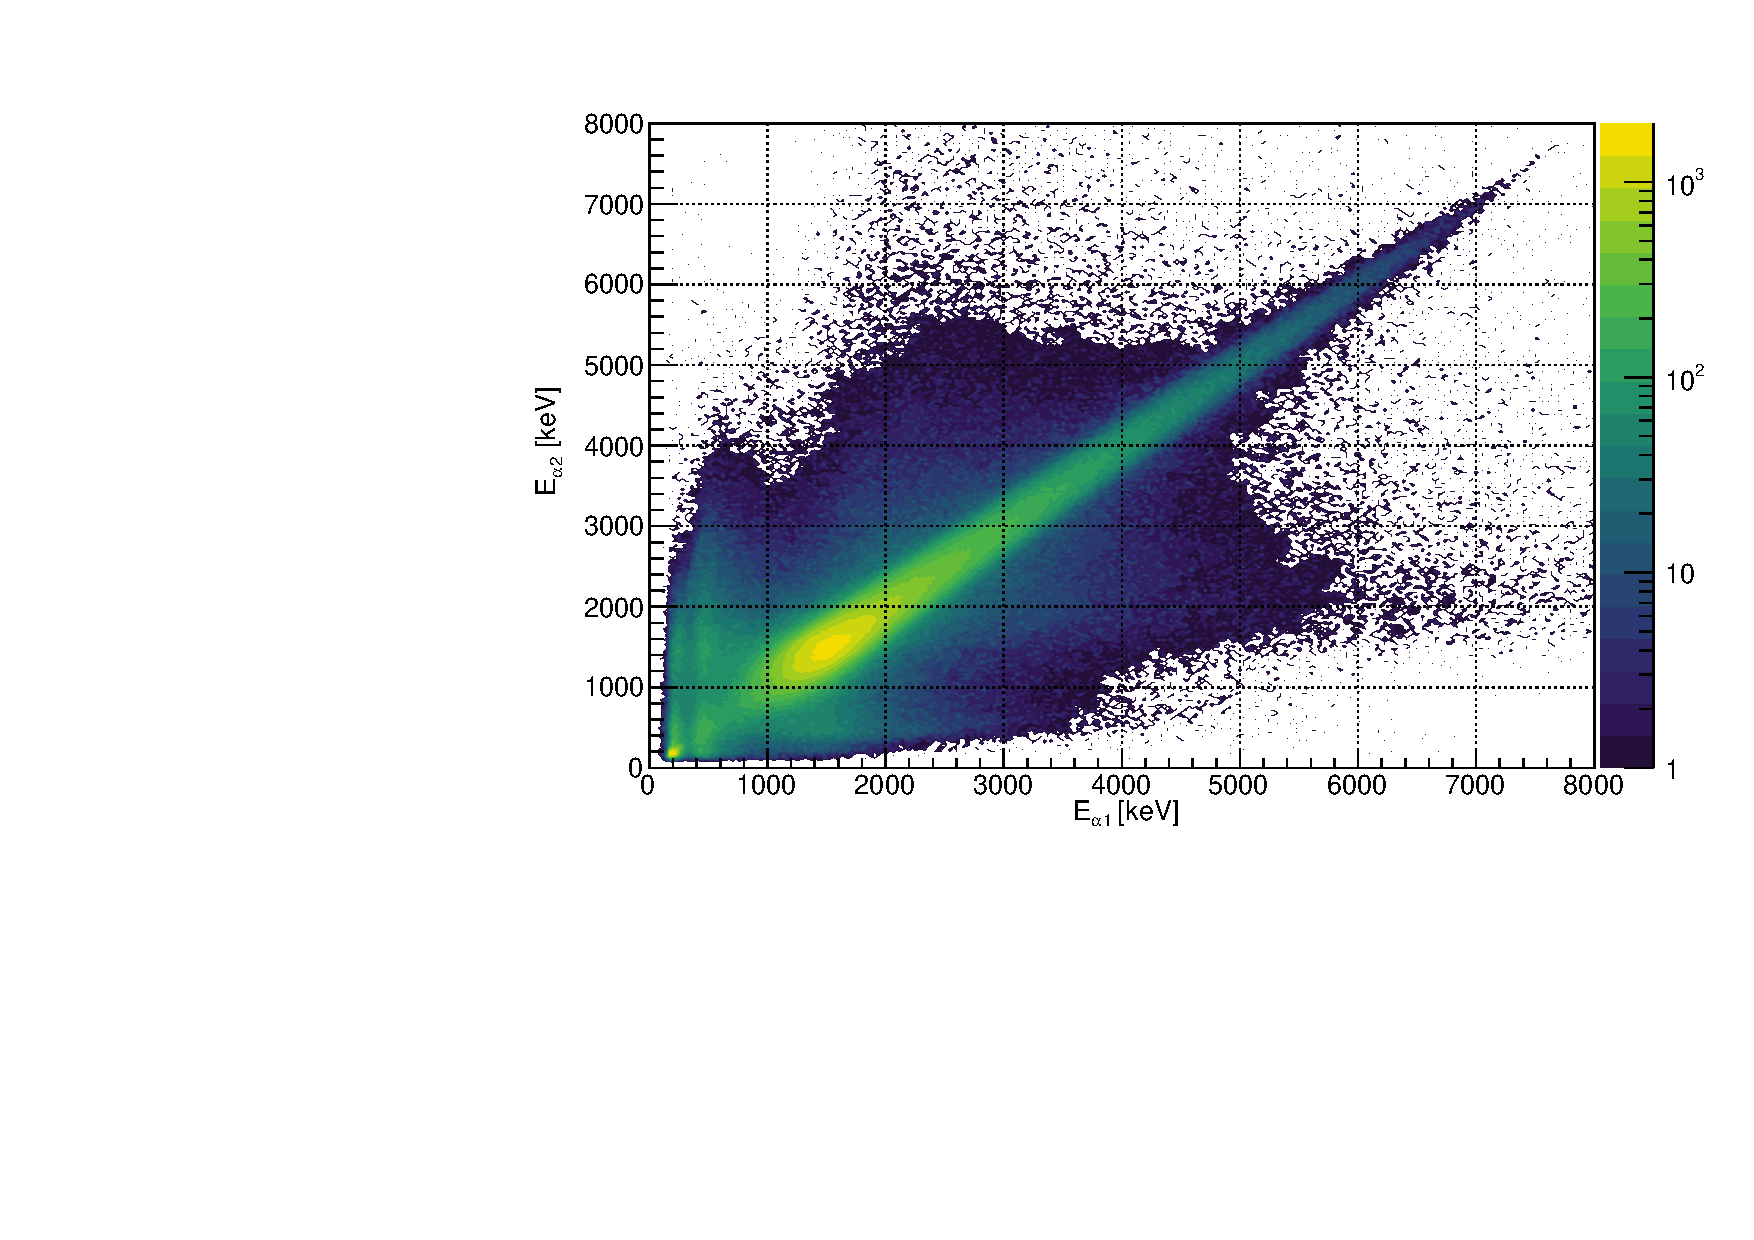
\includegraphics[width=.7\columnwidth]{../figures/EEBetaMulCut.pdf}
	\end{figure}
\end{frame}

\begin{frame}{Effekten af alle cuts}
	Alle cuts 
	\begin{figure}
		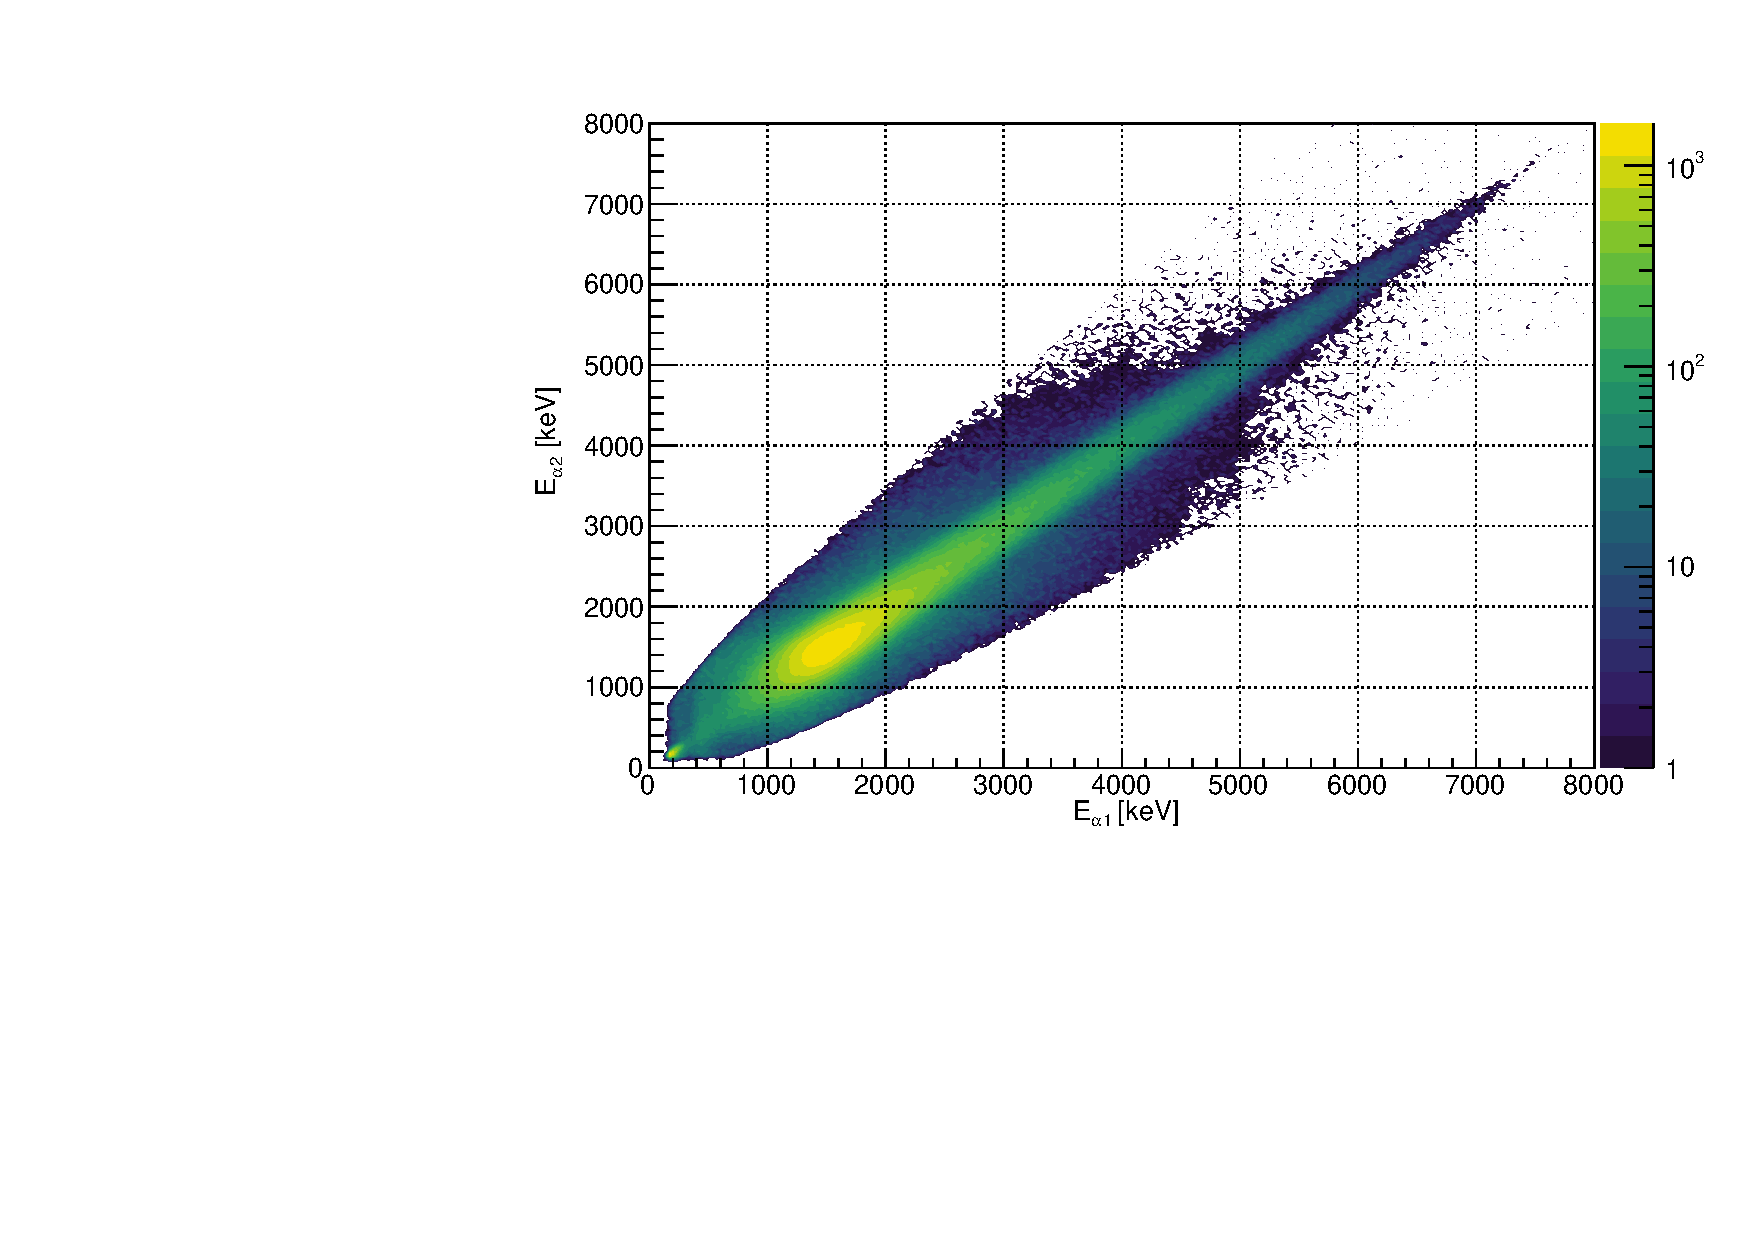
\includegraphics[width=.7\columnwidth]{../figures/EE.pdf}
	\end{figure}
\end{frame}

\begin{frame}{Cut sammenligning}
	Energi spektrum for enkelt \al-partikel
	\begin{figure}
		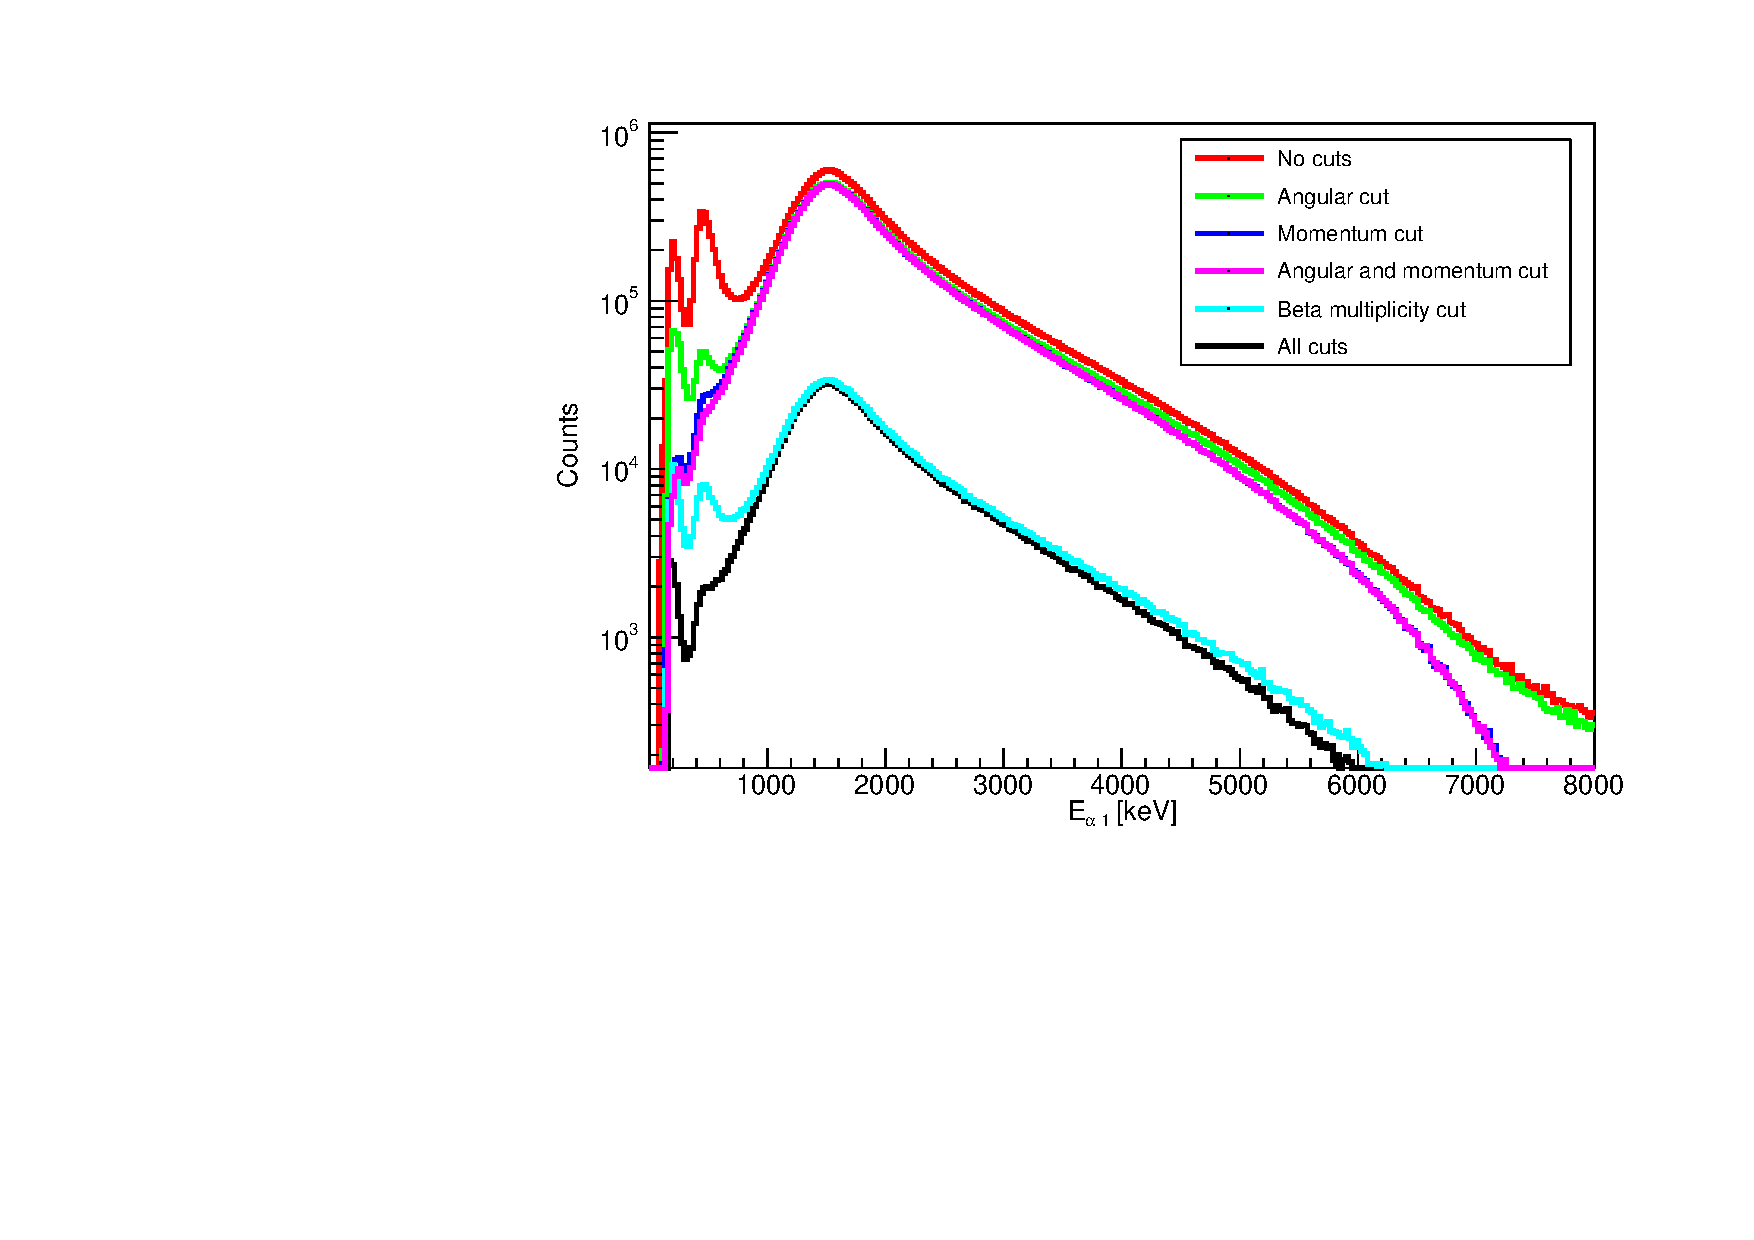
\includegraphics[width=.7\columnwidth]{../figures/cutCompare.pdf}
	\end{figure}
\end{frame}

\begin{frame}{\be\ energi spektrum}
	Falske \be\ identificeringer?
	\begin{figure}
		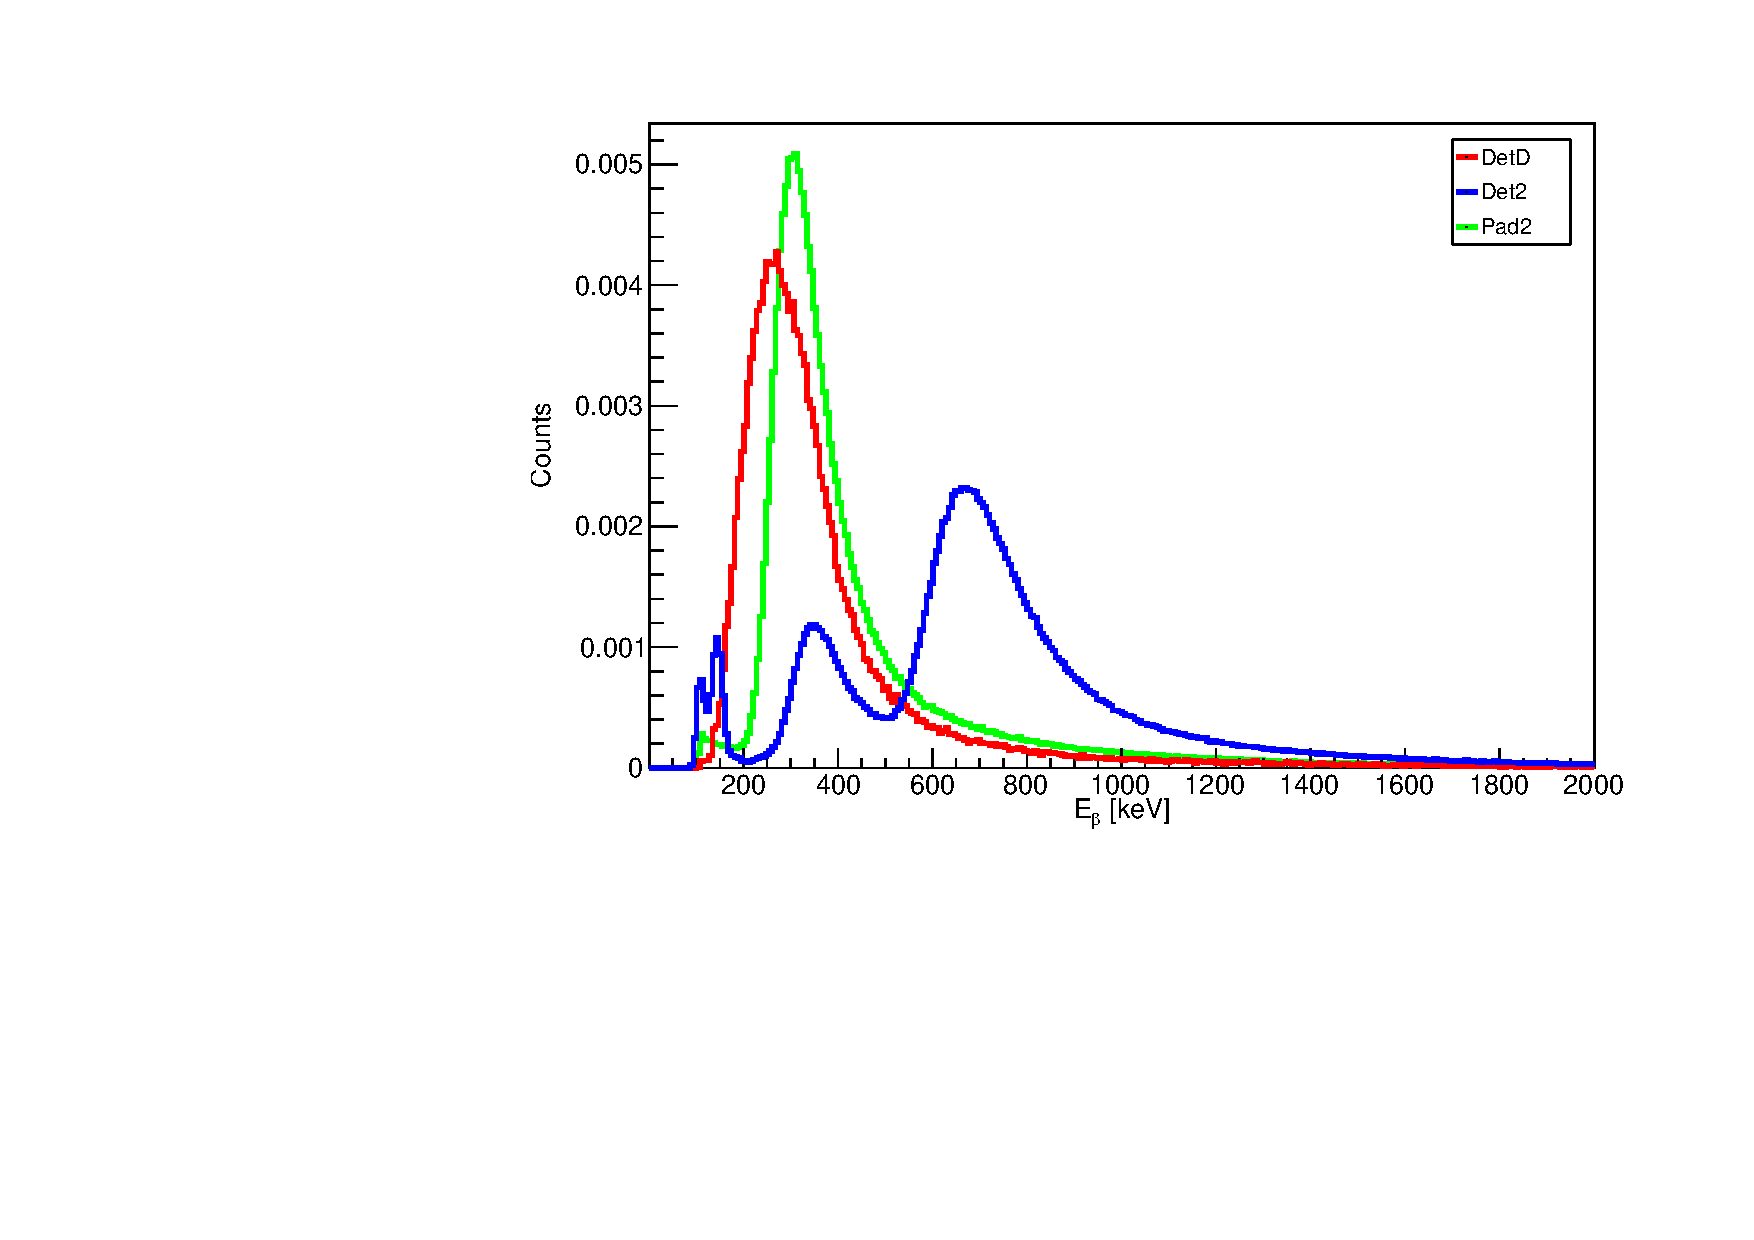
\includegraphics[width=.7\columnwidth]{../figures/betaSpec.pdf}
	\end{figure}
\end{frame}

\section{Data analyse}

\begin{frame}{Excitations spektrum for $^8$Be}
	Energi for summen af to \al-partikler\\
	Sammenligning med tidligere målinger \\
	God overensstemmelse for peak \\
	Lav niveau divagere meget fra hinanden
	\begin{figure}
		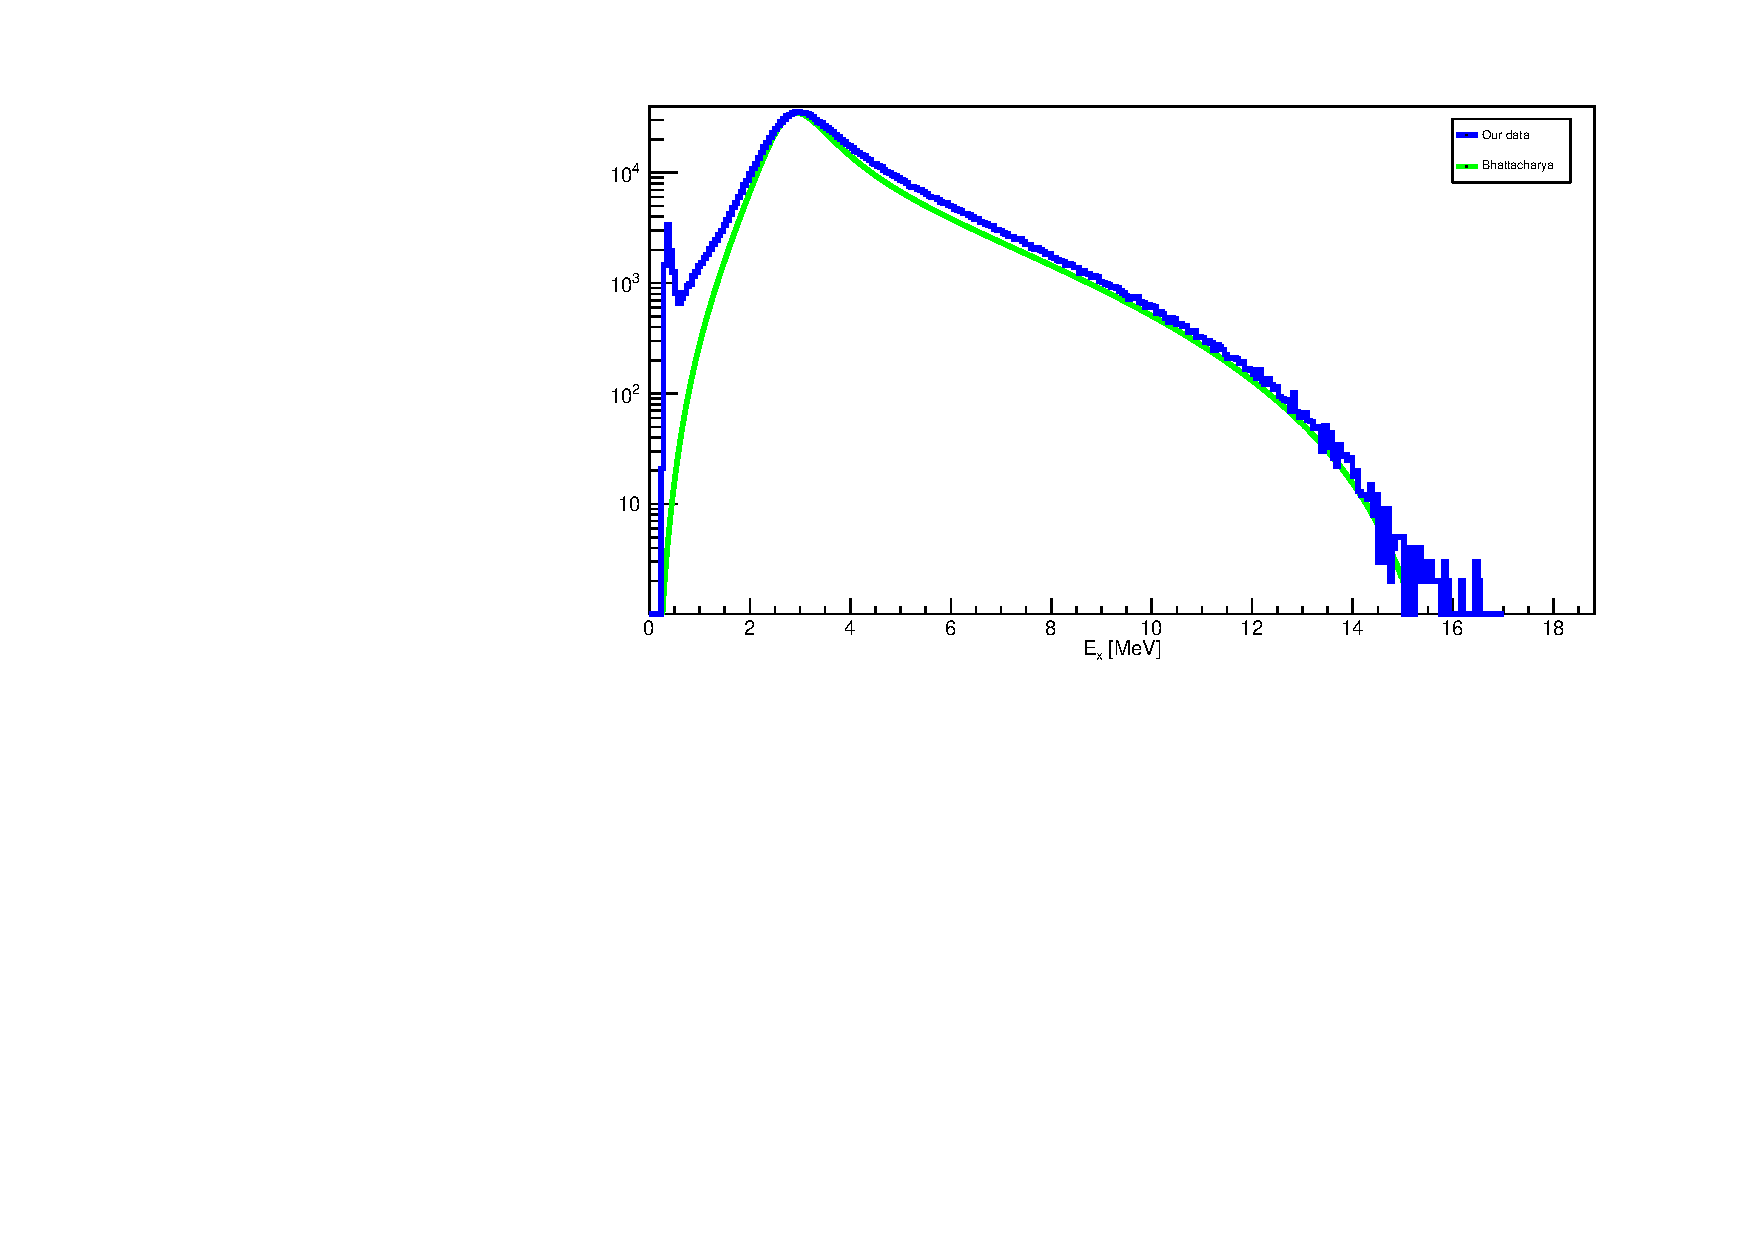
\includegraphics[width=.8\columnwidth]{../figures/bataraCompare.pdf}
	\end{figure}	
\end{frame}

\begin{frame}{Lepton rekyl - måske skip slide?}
	Forskel i energi mellem $\alpha_1$ og $\alpha_2$\\
	Indflydelse på $^8$Be peak\\
	Kan ikke undlades, som forslået af tidligere undersøgelser
	\begin{columns}
		\column[]{0.5\textwidth}\\
		\begin{figure}
			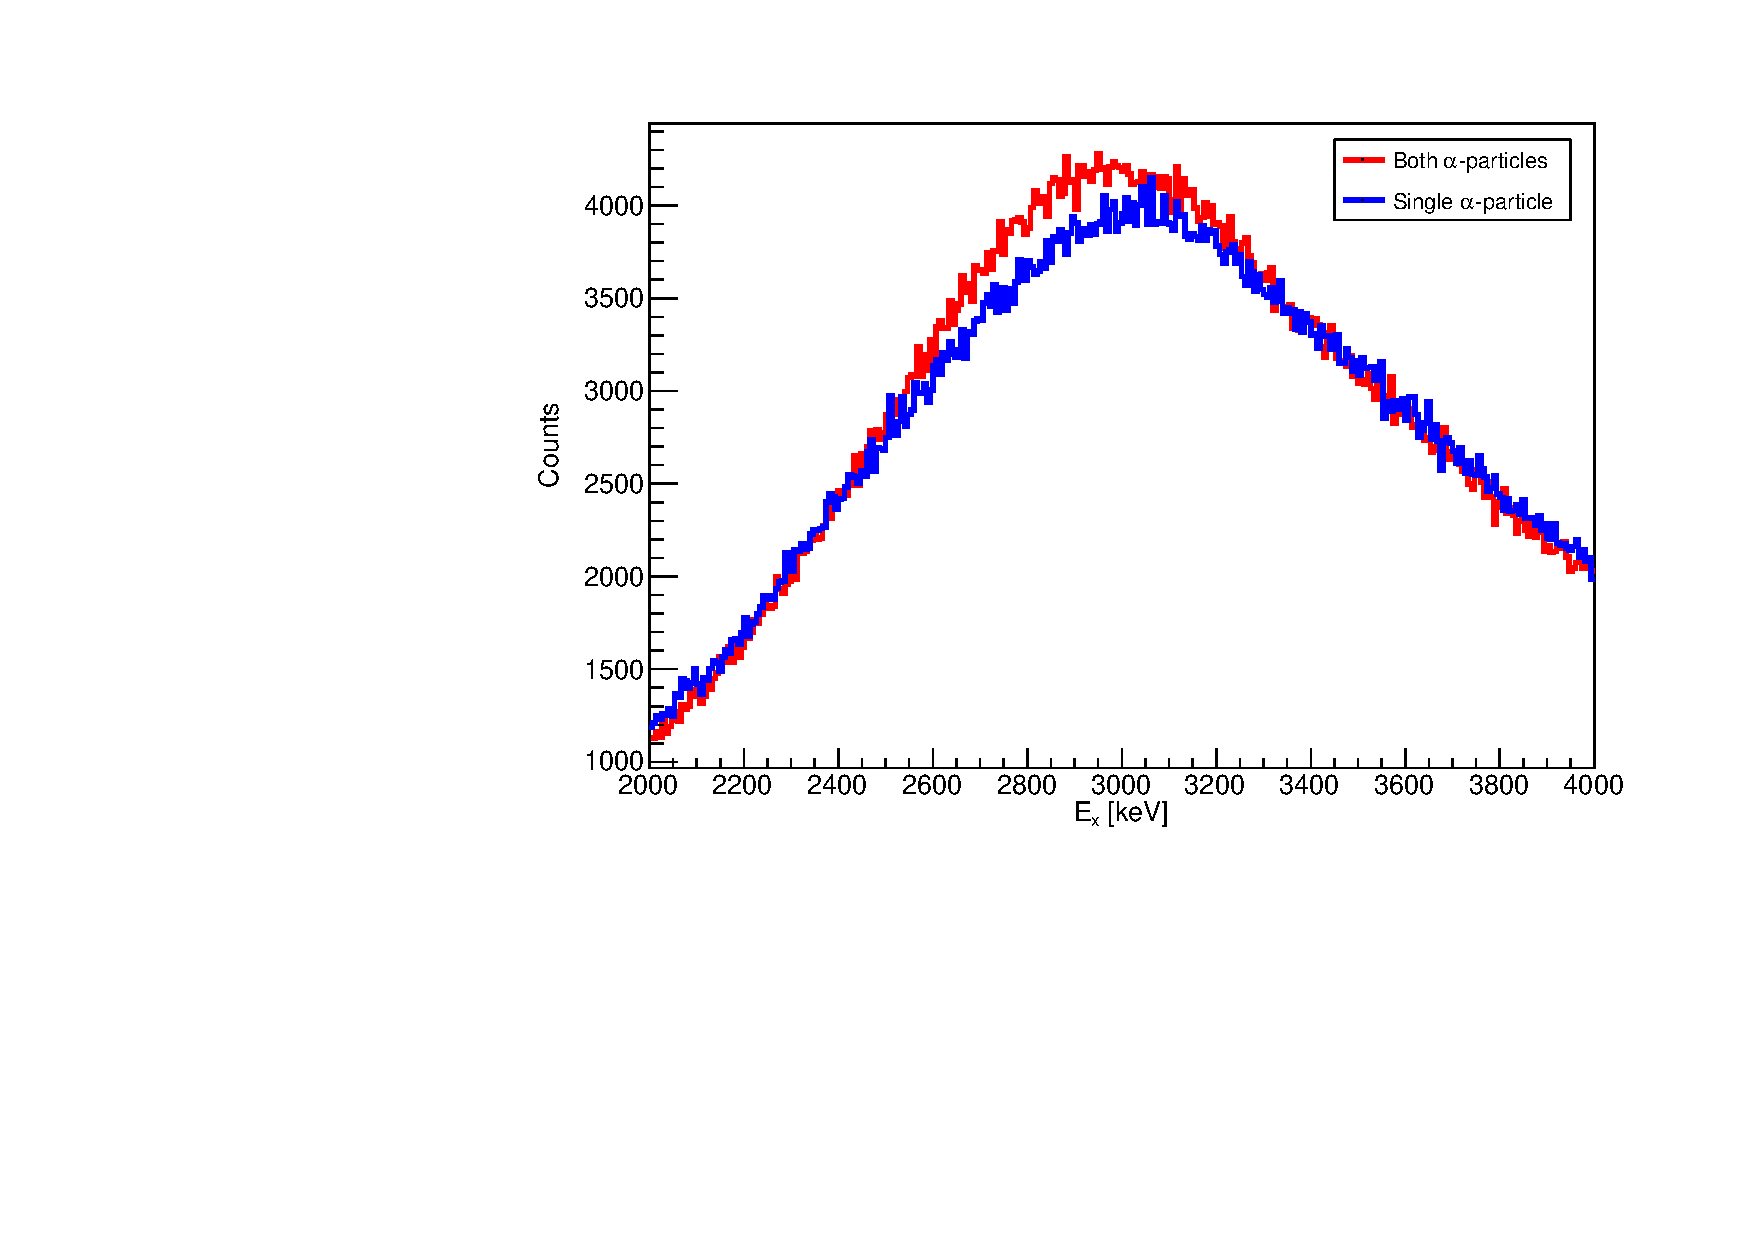
\includegraphics[width=\columnwidth]{../figures/recoil.pdf}
		\end{figure}
		\column[]{0.5\textwidth}\\
		\begin{figure}
			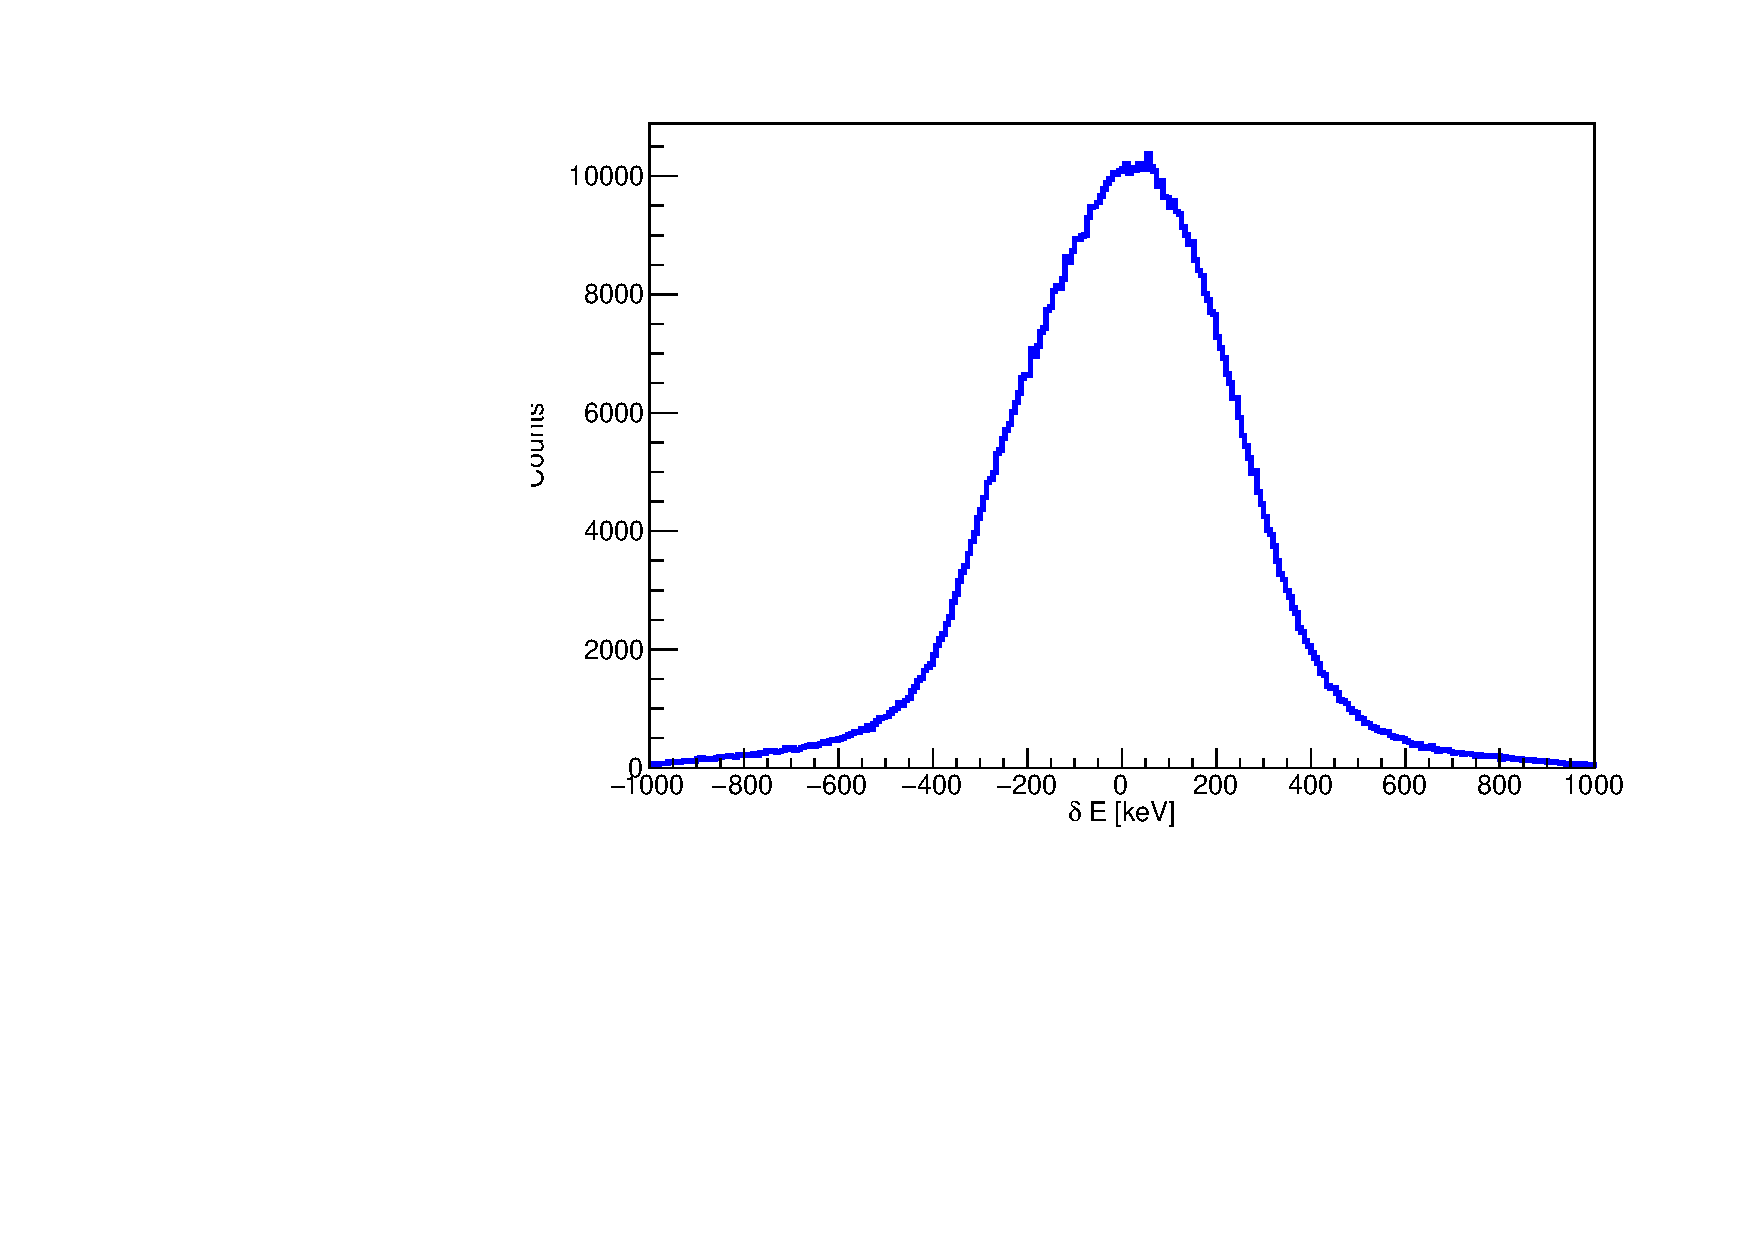
\includegraphics[width=\columnwidth]{../figures/recoilGauss.pdf}
		\end{figure}
	\end{columns}
\end{frame}

\begin{frame}{Vinkel korrelationer mellem \al\ og \be}
\begin{columns}
	\column{0.4\textwidth}
	\begin{itemize}
		\onslide<1->{\item Vinkel mellem $\alpha_1$ og \be\\}
		\onslide<2->{\item Vinkel mellem $\alpha_2$ og \be\\}
		\onslide<3->{\item Giver komplet billede sammenlagt}
		%\onslide<4->{\item Sammenligning med setup effektivitet}
	\end{itemize}
	\column{0.6\textwidth}
	\begin{overprint}
	\onslide<1>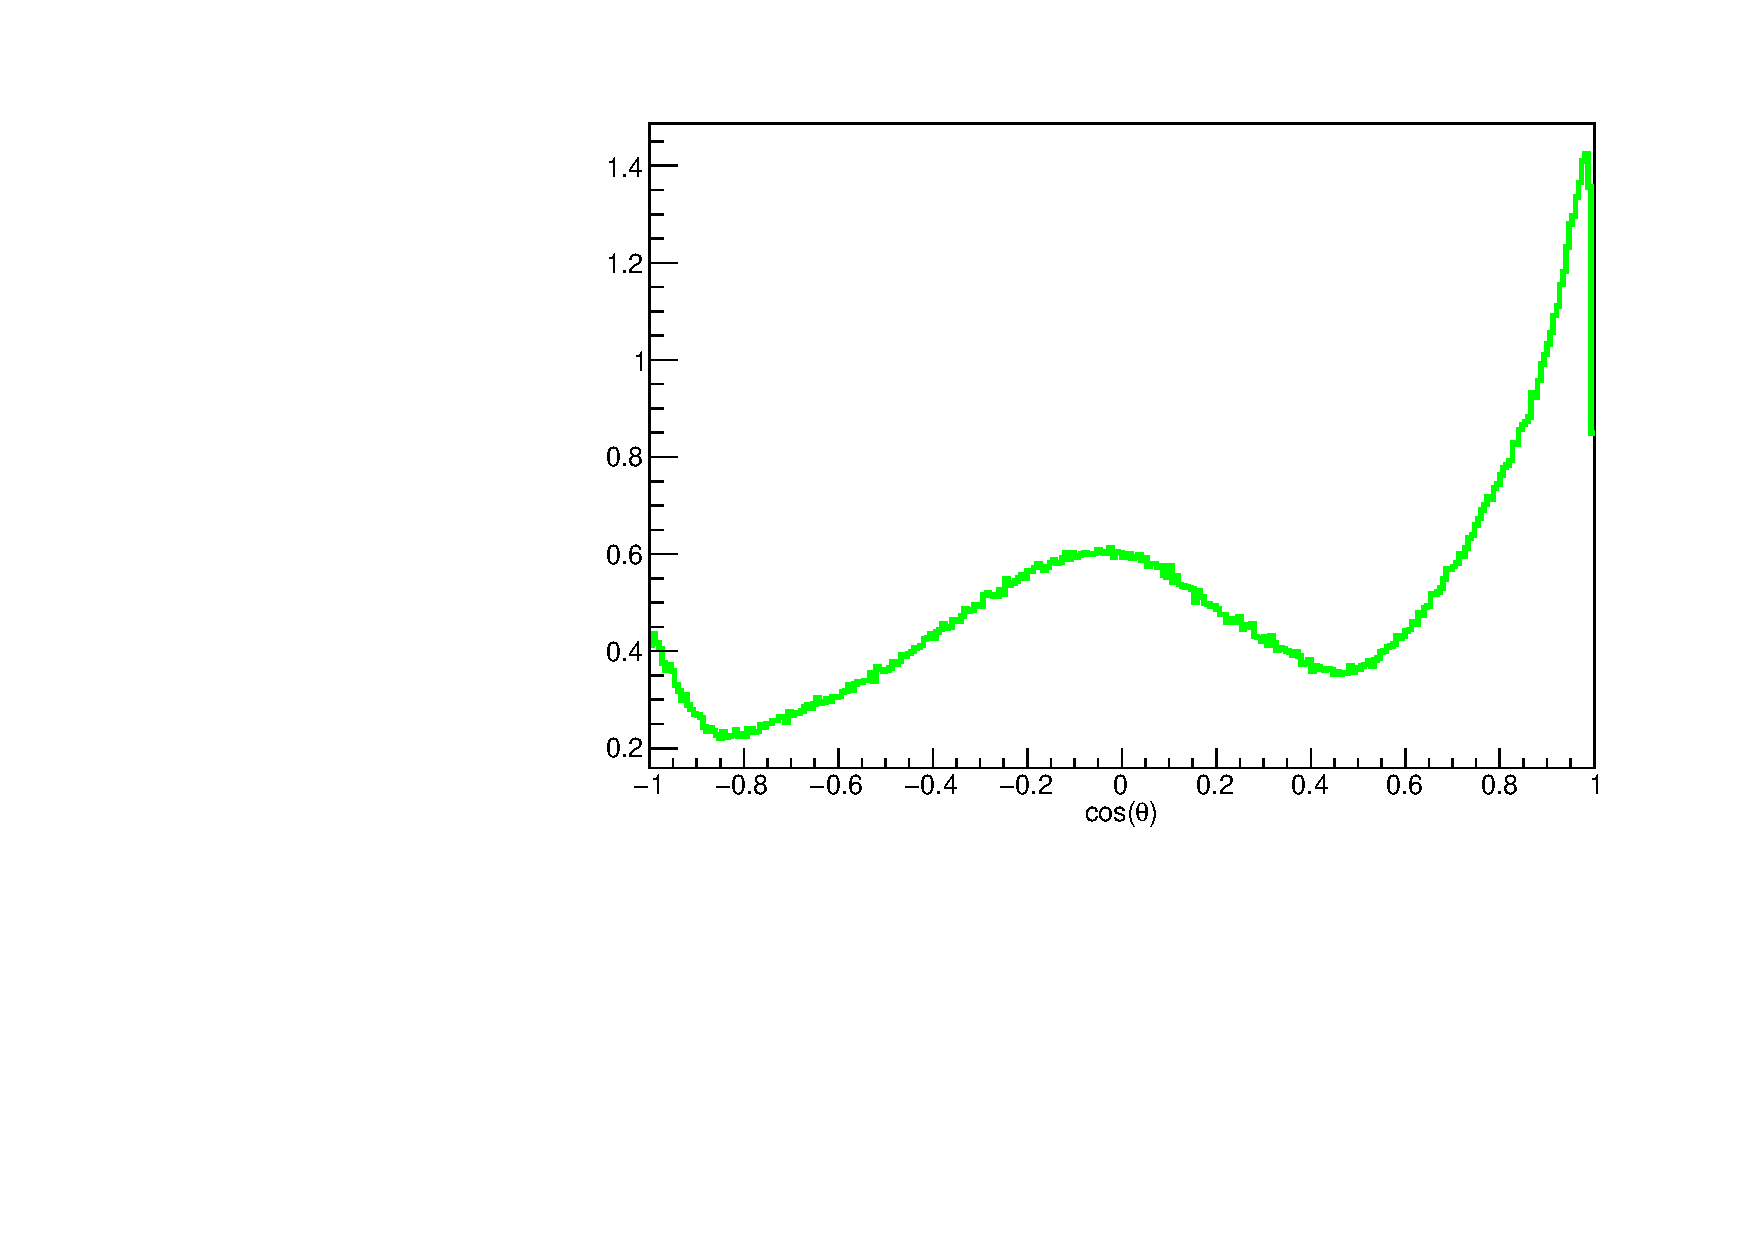
\includegraphics[width=\columnwidth]{../figures/justAl1.pdf}
	\onslide<2>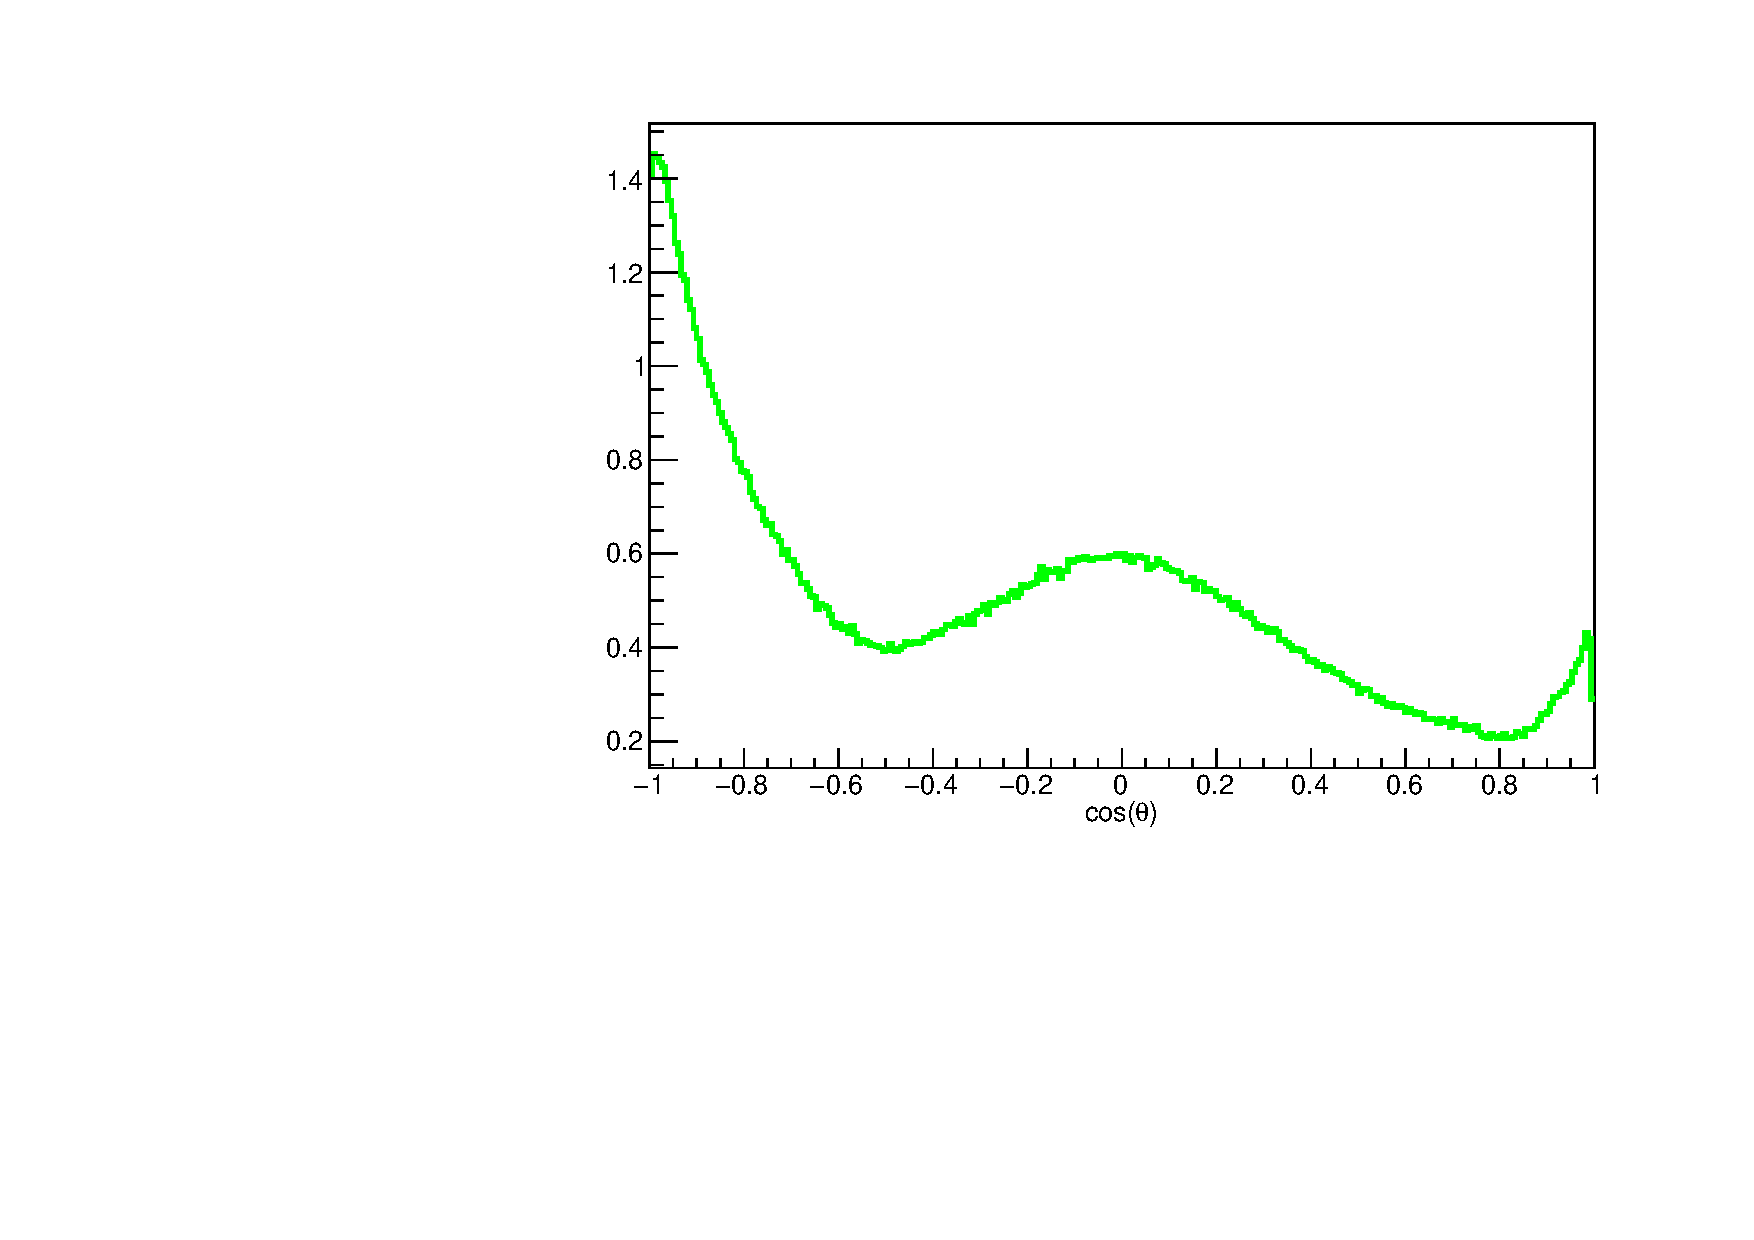
\includegraphics[width=\columnwidth]{../figures/justAl2.pdf}
	\onslide<3>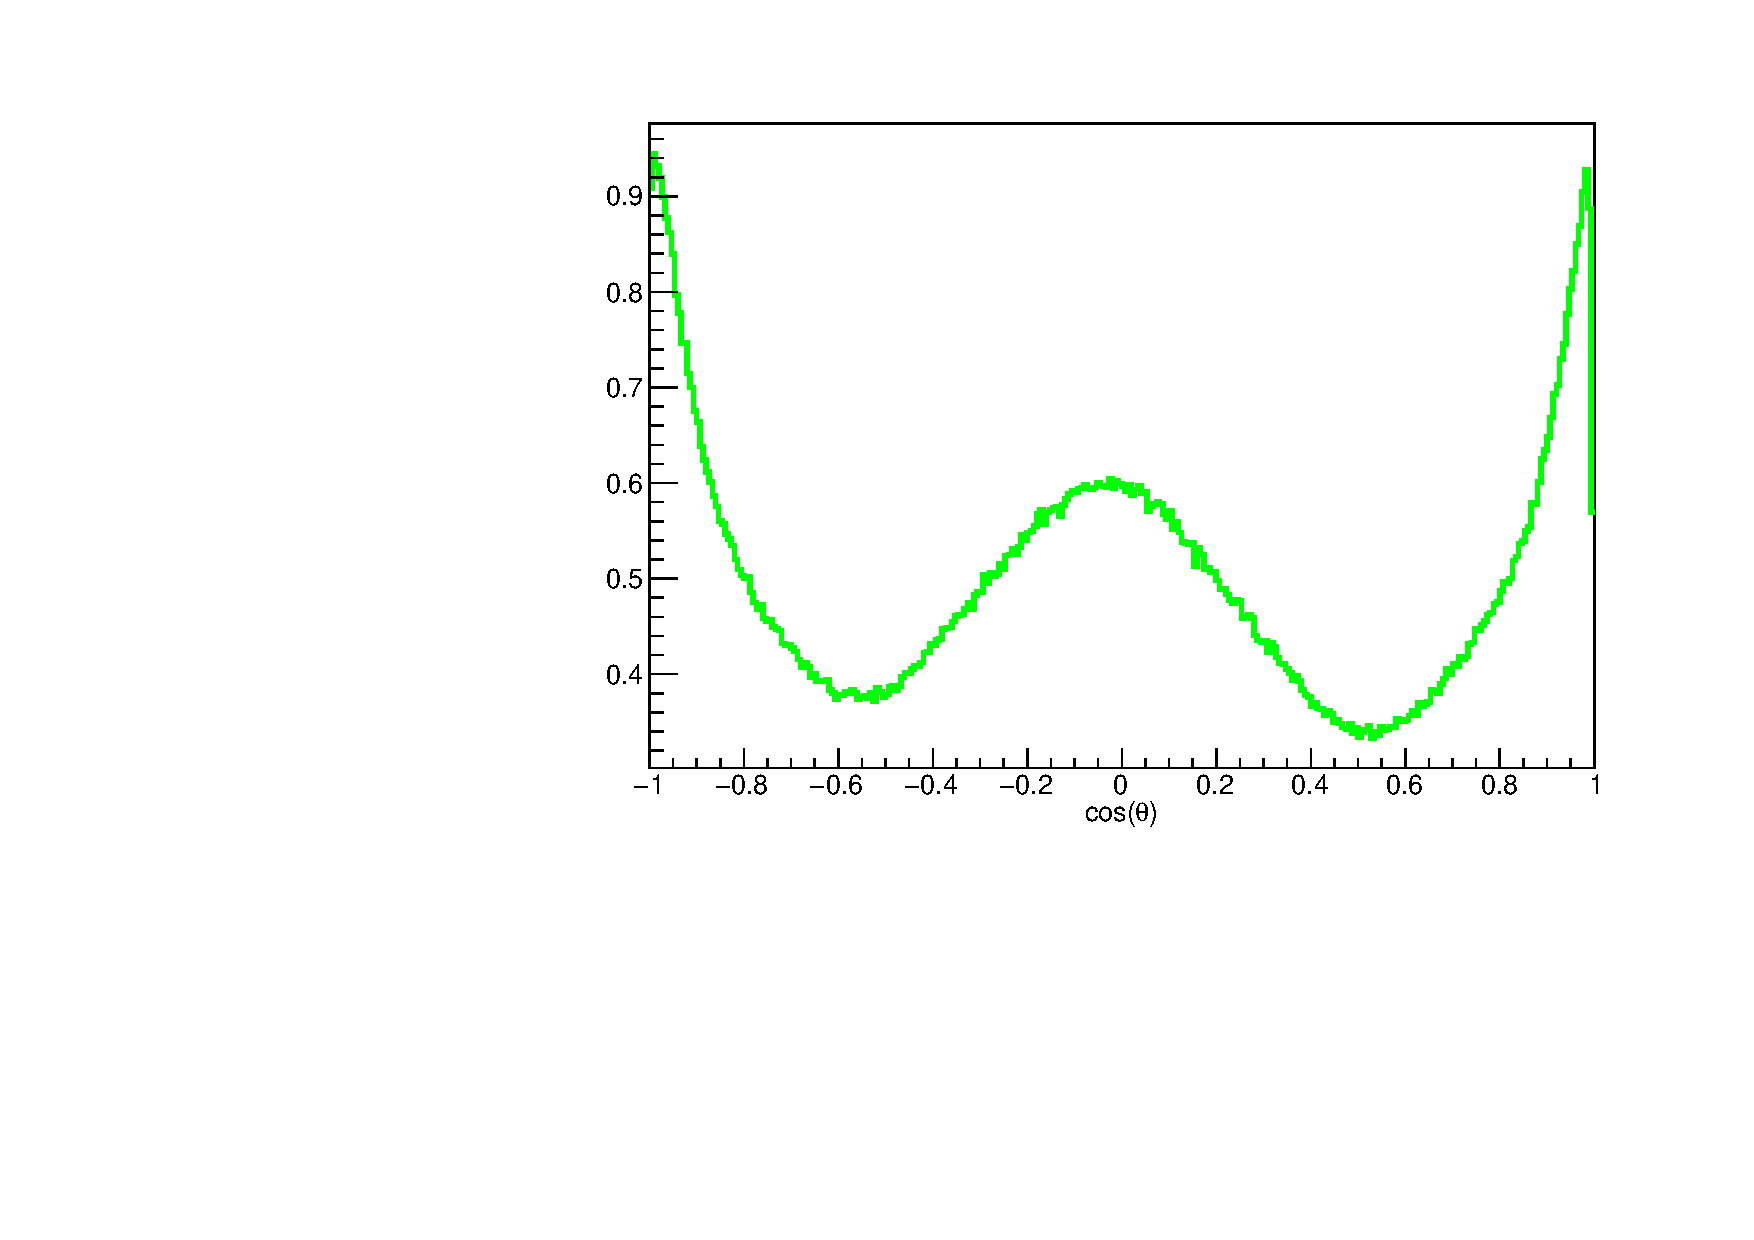
\includegraphics[width=\columnwidth]{../figures/justData.pdf}
	%\onslide<4->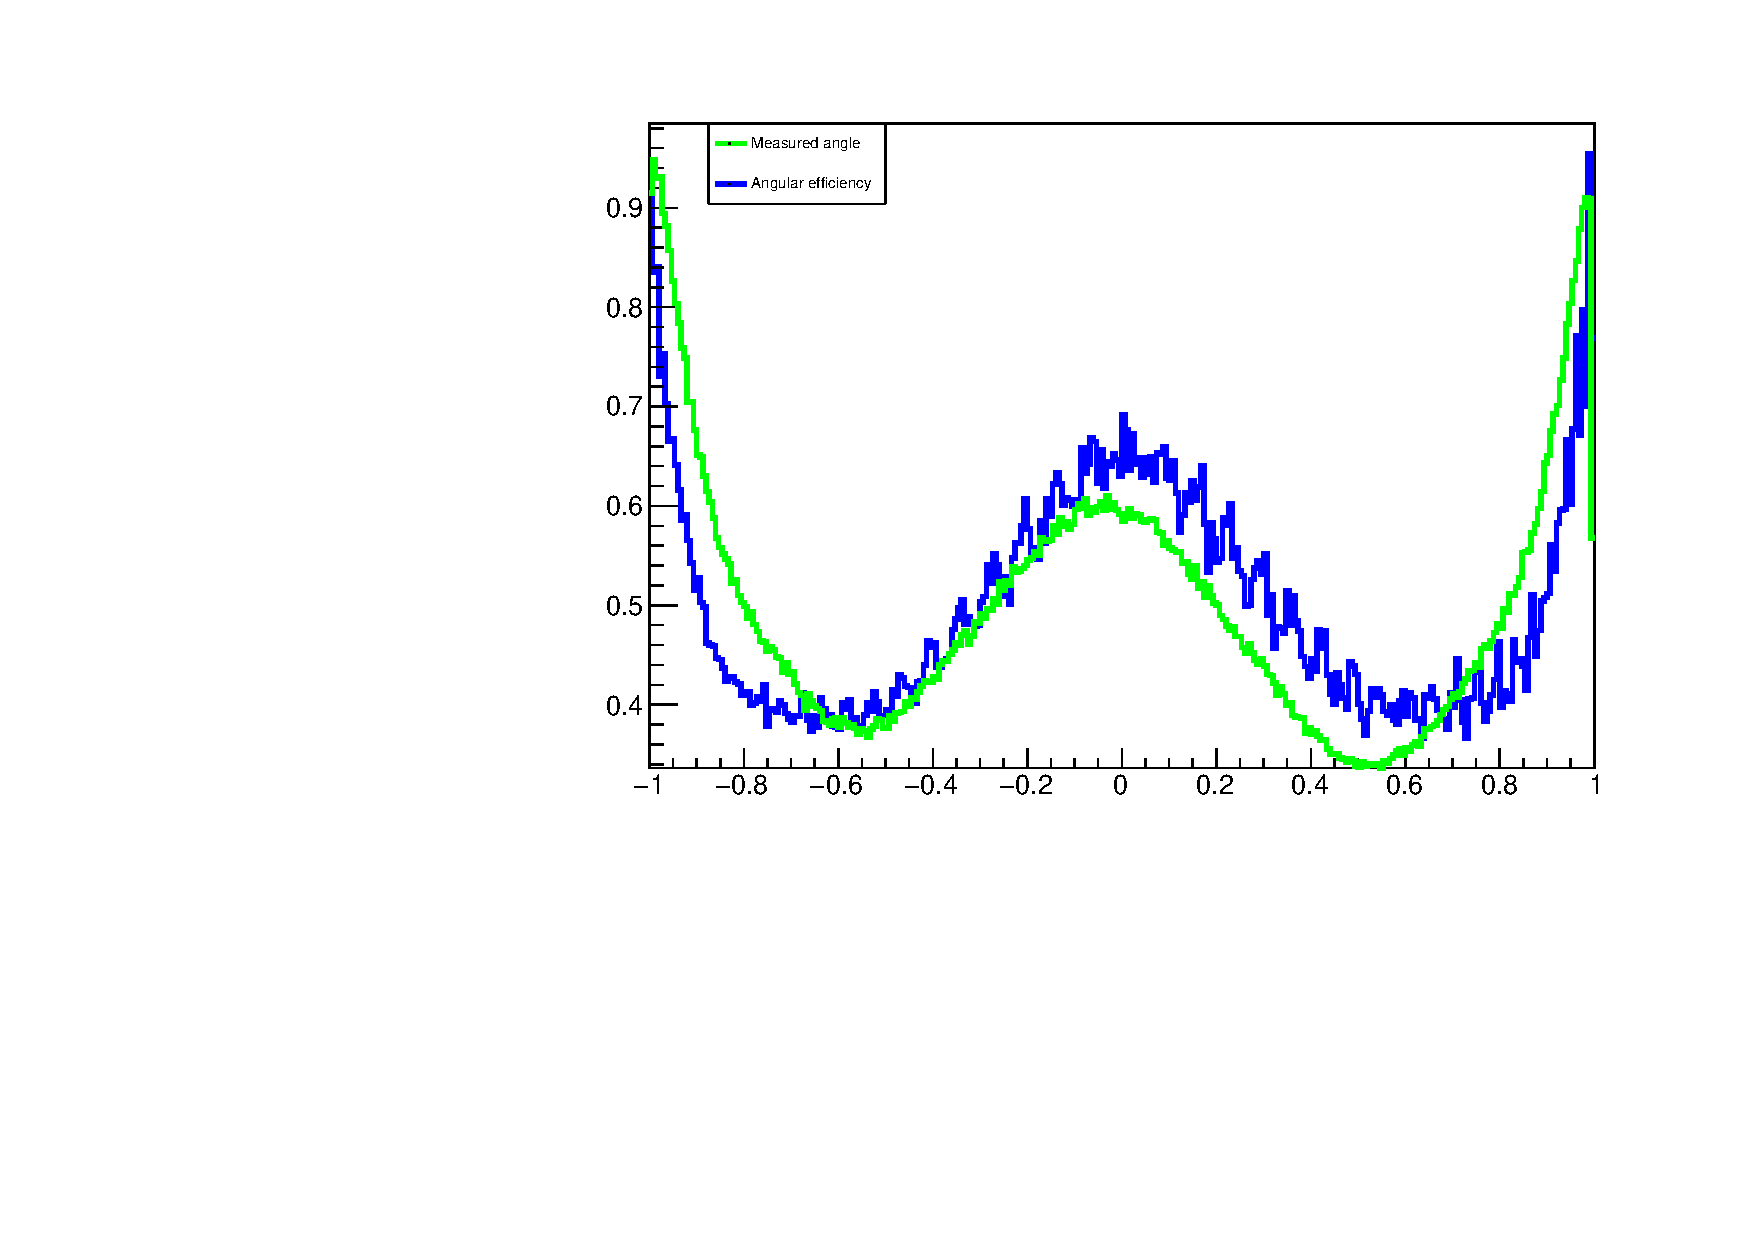
\includegraphics[width=\columnwidth]{../figures/betaAngles/betaAngle.pdf}
	\end{overprint}	
\end{columns}
\end{frame}

\begin{frame}{Setup effektivitet}
	\begin{columns}
		\column[]{.6\textwidth}
		\begin{itemize}
			\onslide<1->{\item Setup har større sandsynlighed for at måle nogle individuelle vinkler\\}
			\onslide<2->{\item Der vil altid være \textcolor{blue}{$180\degree$} mellem en pixel og sig selv\\}
			\onslide<3->{\item Ofte en pixel \textcolor{mypurple}{$90\degree$} eller \textcolor{mypurple}{$180\degree$} fra en given pixel\\}
			\onslide<4->{\item Ikke altid en pixel \textcolor{red}{$45\degree$} eller \textcolor{red}{$135\degree$} fra en pixel}
		\end{itemize}
		
		\column[]{.4\textwidth}
		\begin{overprint}
			\onslide<2>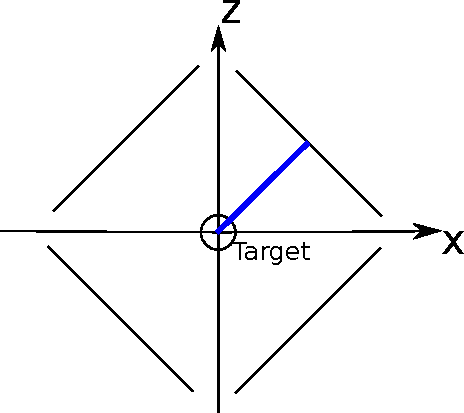
\includegraphics[width=\columnwidth]{../figures/showAngles/opstilling_show_angles_1.pdf}
			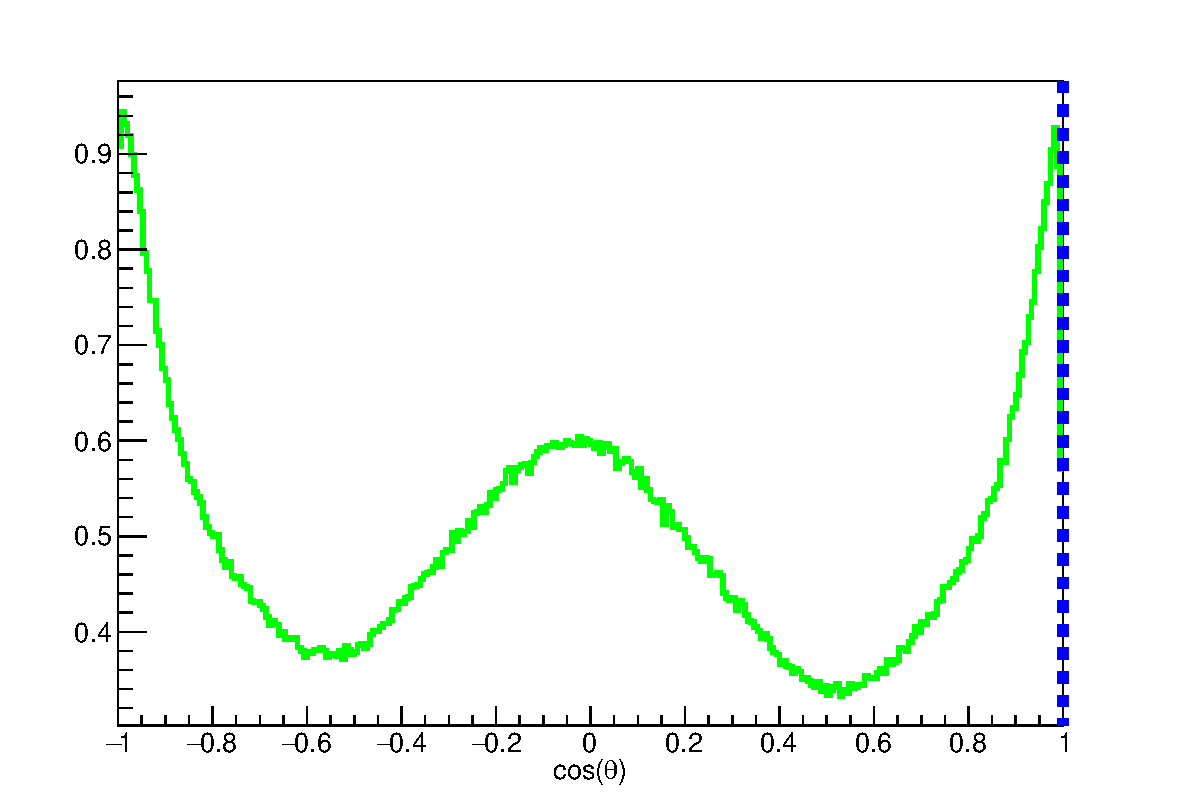
\includegraphics[width=\columnwidth]{../figures/showAngles/data_1.pdf}
			\onslide<3>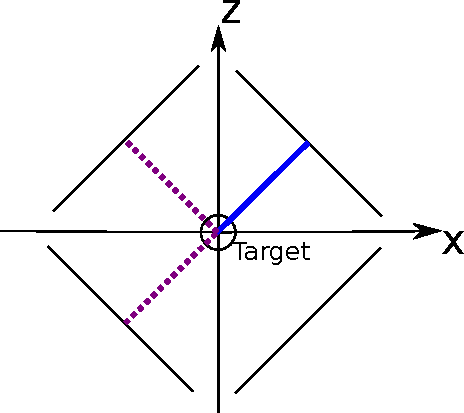
\includegraphics[width=\columnwidth]{../figures/showAngles/opstilling_show_angles_2.pdf}
			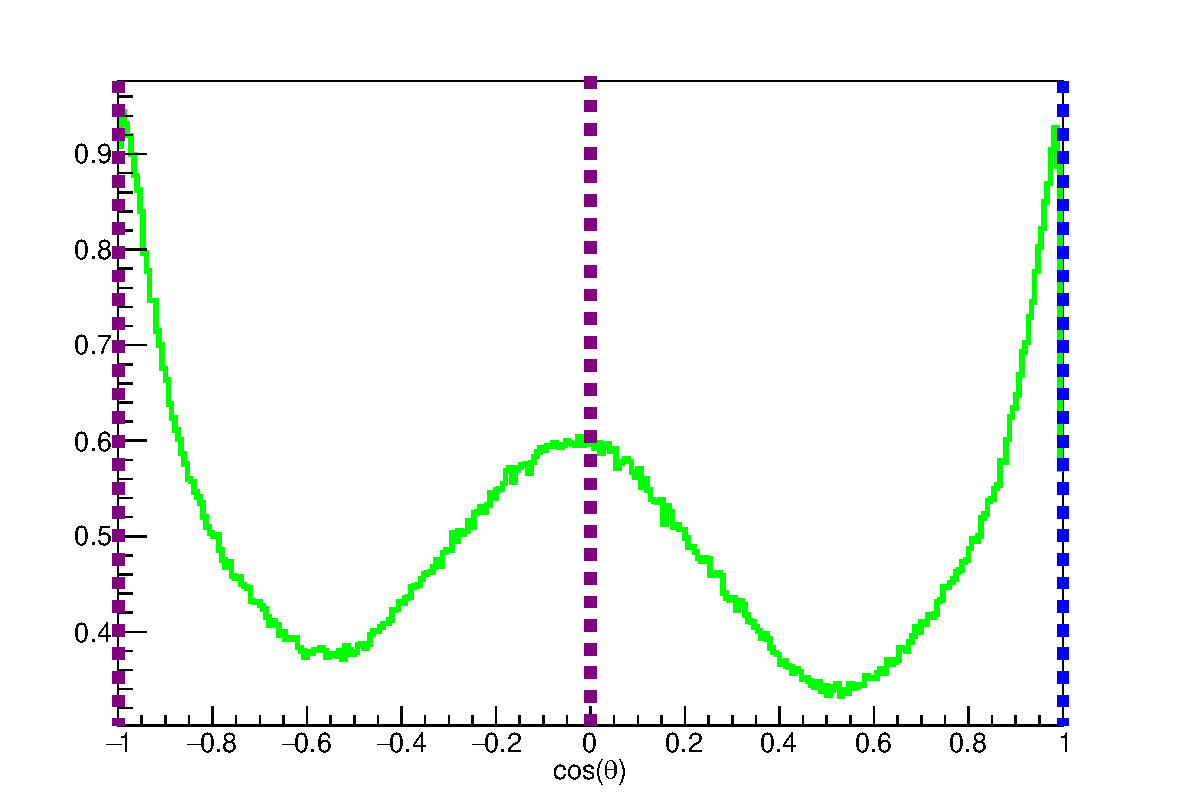
\includegraphics[width=\columnwidth]{../figures/showAngles/data_2.pdf}
			\onslide<4->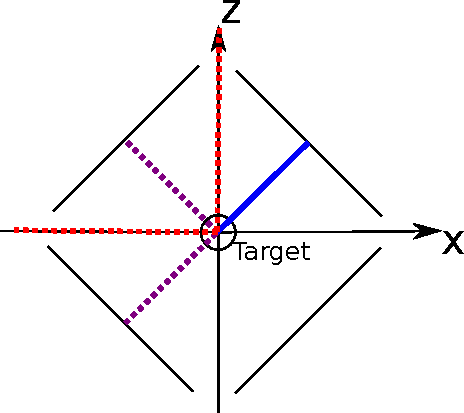
\includegraphics[width=\columnwidth]{../figures/showAngles/opstilling_show_angles_3.pdf}
			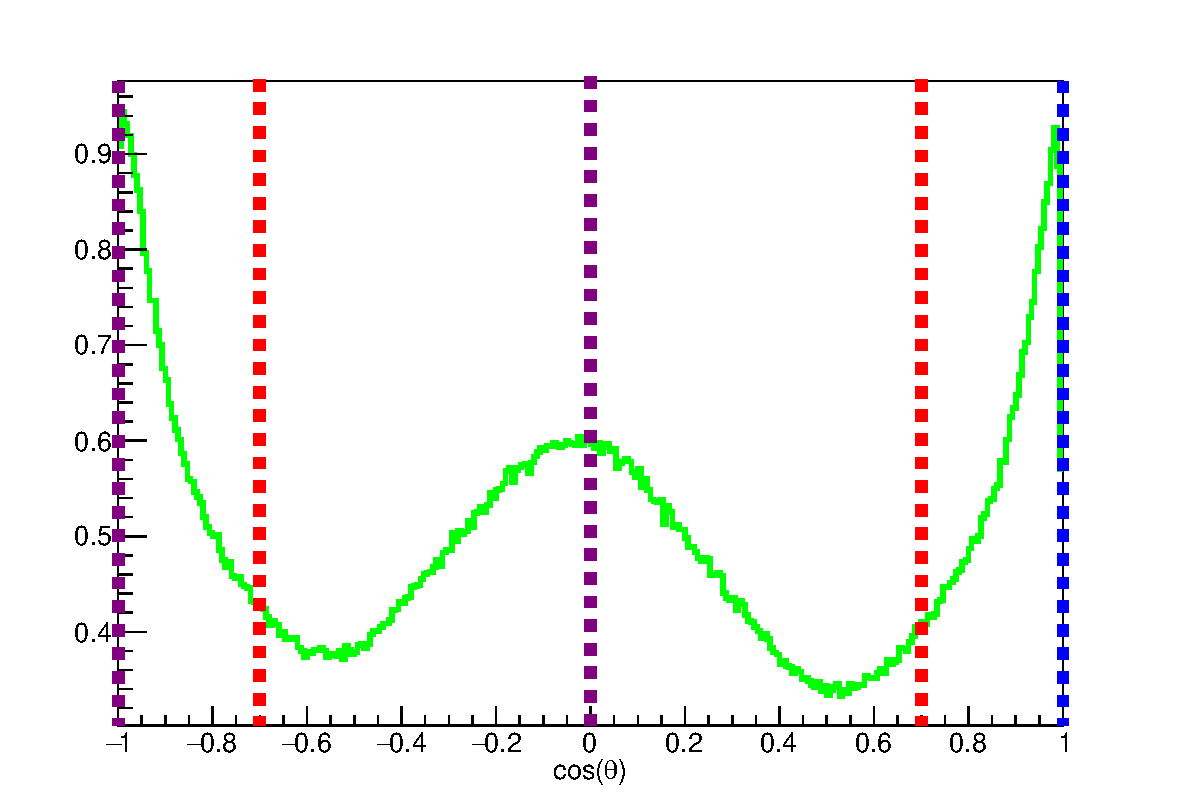
\includegraphics[width=\columnwidth]{../figures/showAngles/data_3.pdf}
		\end{overprint}
	\end{columns}
\end{frame}

\begin{frame}{Setup effektivitet}
	\begin{itemize}
		\item Udregn den forventede vinkelfordeling
		\item Vinklen mellem en pixel $i$ i en hvilken som helst detektor, og en anden pixel $j$ i en given detektor
	\end{itemize}
	\begin{figure}
		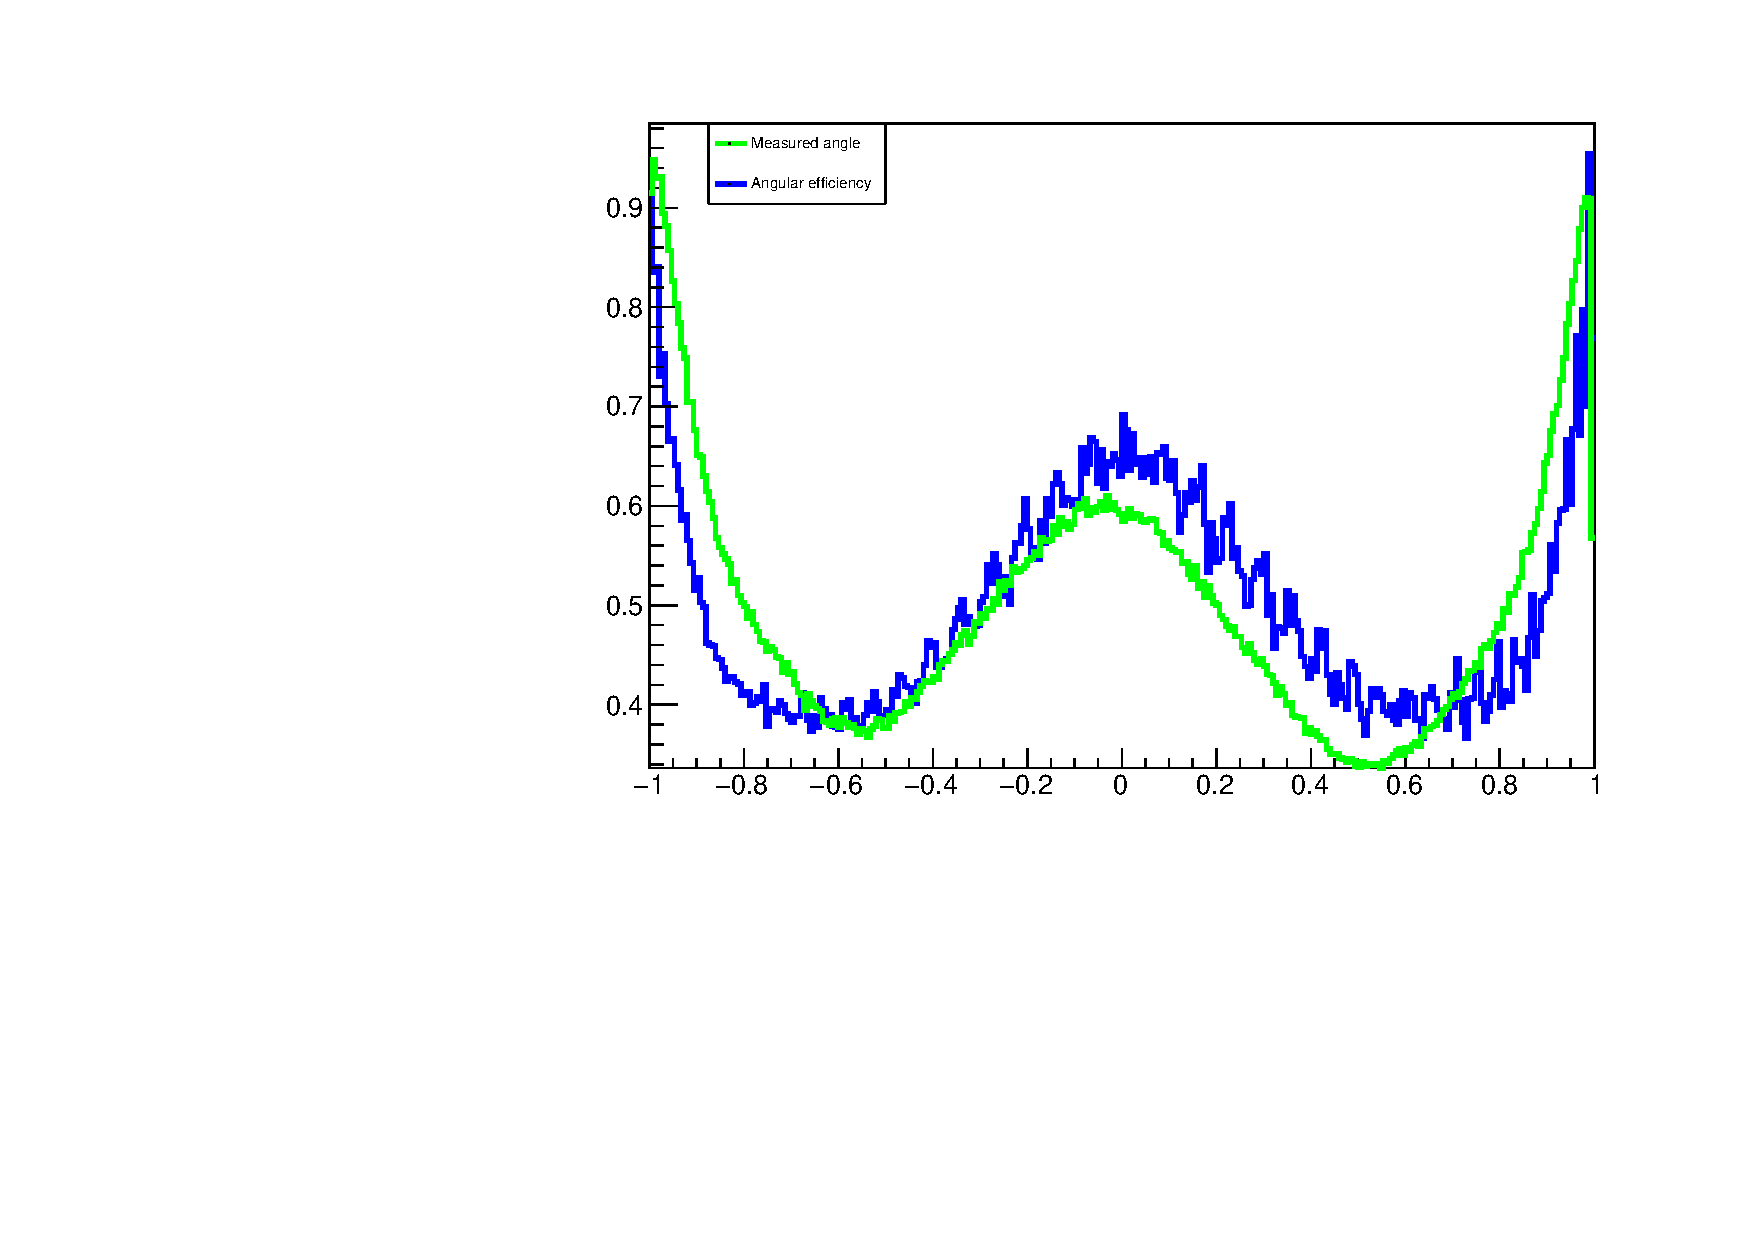
\includegraphics[width=0.7\columnwidth]{../figures/betaAngles/betaAngle.pdf}
	\end{figure}
\end{frame}